% This is my thesis, read it first and I will ask questions
% later also in comments. 

\documentclass[a4paper,12pt]{article}

\setlength{\textwidth}{15.0cm}
\setlength{\textheight}{24.0cm}
\setlength{\topmargin}{0cm}
\setlength{\headsep}{0cm}
\setlength{\headheight}{0cm}
\pagestyle{plain}


\usepackage{hyperref}
\hypersetup{
    colorlinks=true,
    linkcolor=blue,
    filecolor=magenta,      
    urlcolor=blue,
    citecolor=blue,
    linktoc=page
}
\usepackage[dvips]{epsfig}
\usepackage{tikz}
\usepackage[english]{babel}
\usepackage{caption}
\captionsetup{font=it}

\usepackage[
backend=biber,
style=alphabetic,
]{biblatex}

\renewcommand{\bibfont}{\footnotesize}


\usepackage{amsmath,amssymb,amsthm}
\newtheoremstyle{break}{4pt}{4pt}{}{}{\bfseries}{\vspace{2 pt}}{\newline}{}
\theoremstyle{break}
\newtheorem{theorem}{Theorem}[subsection]
\newtheorem{example}[theorem]{Example}
\newtheorem{definition}[theorem]{Definition}
\newtheorem{notation}[theorem]{Notation}
\newtheorem{lemma}[theorem]{Lemma}
\newtheorem{corollary}[theorem]{Corollary}
\newtheorem{technique}[theorem]{Technique}
\newtheorem{pythonn}[theorem]{Python Code}
\newtheorem{related}[theorem]{Related Work}

\usepackage{comment}
\usepackage{listings}
% Define custom colors for Python syntax highlighting
\definecolor{codebackground}{RGB}{242, 242, 242}
\definecolor{codecomment}{RGB}{106, 153, 85}
\definecolor{codekeyword}{RGB}{0, 0, 255}
\definecolor{codestring}{RGB}{170, 55, 241}

% Define custom Python style for syntax highlighting
\lstdefinestyle{custompython}{
    language=Python,
    backgroundcolor=\color{codebackground},
    basicstyle=\ttfamily\footnotesize,
    commentstyle=\color{codecomment}\itshape,
    keywordstyle=\color{codekeyword}\bfseries,
    stringstyle=\color{codestring},
    showstringspaces=false,
    breaklines=true,
    breakatwhitespace=true,
    tabsize=4,
    frame=tb,
    framesep=4pt,
    framerule=0.5pt,
    numbers=left,
    numbersep=10pt,
    numberstyle=\footnotesize\color{gray},
    xleftmargin=15pt,
    xrightmargin=5pt,
    aboveskip=5pt,
    belowskip=5pt,
    captionpos=b
}

\newcommand{\pythoncode}[1]{
    \hspace*{0cm}
    \vspace{-0.3cm}
    \lstinputlisting[style=custompython]{#1}}

% Define custom colors for Julia syntax highlighting
\definecolor{juliabackground}{RGB}{240, 230, 255} % Light purple background
\definecolor{juliacomment}{RGB}{128, 0, 128}     % Purple comments
\definecolor{juliakeyword}{RGB}{75, 0, 130}      % Indigo keywords
\definecolor{juliastring}{RGB}{147, 112, 219}    % Medium purple strings

% Define custom Julia style for syntax highlighting
\lstdefinelanguage{Julia}%
{
    morekeywords={
            abstract, break, case, catch, const, continue, do, else, elseif, end,
            export, false, for, function, global, if, immutable, import, importall,
            in, macro, module, otherwise, quote, return, switch, true, try, type,
            typealias, using, while
        },
    sensitive=true,
    alsoother={$},
    morecomment=[l]\#,
    morecomment=[n]{\#=}{=\#},
    morestring=[s]{"}{"},
    morestring=[s]{'}{'},
}[keywords,comments,strings]

\lstdefinestyle{customjulia}{
    language=Julia,
    backgroundcolor=\color{juliabackground},
    basicstyle=\ttfamily\footnotesize,
    commentstyle=\color{juliacomment}\itshape,
    keywordstyle=\color{juliakeyword}\bfseries,
    stringstyle=\color{juliastring},
    showstringspaces=false,
    breaklines=true,
    breakatwhitespace=true,
    tabsize=4,
    frame=tb,
    framesep=4pt,
    framerule=0.5pt,
    numbers=left,
    numbersep=10pt,
    numberstyle=\footnotesize\color{gray},
    xleftmargin=15pt,
    xrightmargin=5pt,
    aboveskip=5pt,
    belowskip=5pt,
    captionpos=b,
    columns=flexible,
    keepspaces=true
}

\newcommand{\juliacode}[1]{
    \hspace*{0cm}
    \vspace{-0.3cm}
    \lstinputlisting[style=customjulia]{#1}
}

\addbibresource{bibliography2.bib} 
\setlength{\parindent}{0pt}

\selectlanguage{English}
\begin{document}

\begin{titlepage}
    \begin{center}
        \resizebox{3cm}{!}{
\includegraphics{./vert2_kl_01.eps}}
        \ \
        \ \\
        \ \\
        \ \\
        \ \\
        \ \\
        \ \\
        \ \\
        \ \\
        \ \\
        \ \\
        \ \\
        \Large{M{\sc asterproef scriptie}}
        \ \\
        \ \\
        \ \\
        \huge{\bf{\em Recursive Monte Carlo for linear ODEs}}
        \ \\
        \ \\
        \ \\
        % \ \\
        \ \\
        \ \\
        \normalsize
        Auteur: {\em Isidoor Pinillo Esquivel}\\
        \ \\
        \ \\
        Promotor: {\em Wim Vanroose}\\
        \ \\
        \ \\
        \ \\
        \ \\
        \ \\
        \ \\
        \ \\
        A{\sc cademiejaar 2022-2023}

    \end{center}
\end{titlepage}




\newpage
\tableofcontents
\newpage

\begin{abstract}
    Unbiased algorithms for solving linear initial value problems have received limited attention.
This is addressed here by proposing unbiased Recursive Monte Carlo methods for solving
linear initial value problems and linear Fredholm integral equations of the second kind. Motivated
by understanding randomized parallel complexity and downstream applications to partial differential
equations, these methods are developed.

Previously only biased methods were known to achieve optimal convergence rates for nonlinear
initial value problems which has primarily theoretical significance.
The proposed RRMC method, an unbiased algorithm for linear initial value problems,
together with control variates is conjectured to be order optimal with high
probability for corresponding smoothness classes.

Parallel to this, the main Poisson algorithm is proposed, generalizing the algorithm in \cite{acebron_monte_2016},
which is simple and forward implementable. The main Poisson algorithm is applied
to the semi-discretized heat equation demonstrating a path resampling technique, that provides
a novel perspective on the Walk on Spheres method, with potential for alternative generalizations.

The proposed methods broadens the understanding of what is possible with unbiased algorithms for
solving linear initial value problems, paving the way for further research in this area.
\end{abstract}


\section{Introduction}

\subsection{Related Work}
The primary motivating paper for this work is the work
by \citeauthor{sawhney_grid-free_2022}
(\citeyear{sawhney_grid-free_2022}) \cite{sawhney_grid-free_2022},
which introduces the Walk-on-Sphere (WoS) method for solving second-order
elliptic PDEs with varying coefficients and Dirichlet boundary conditions.
Their techniques have shown high accuracy even in the presence of geometrically
complex boundary conditions. We were inspired to apply the underlying
mechanics of these Monte Carlo (MC) techniques to ODEs to explore
parallel in time and the possibility of extending their techniques
to other types of PDEs. \\

We made an interactive data map of the literature read
mainly in the function of this thesis available at
\url{https://huggingface.co/spaces/ISIPINK/zotero_map}.
It may take 10 seconds to load. \\

The latest paper that we found on an unbiased Initial Value Problem (IVP) solver is by
\citeauthor{ermakov_monte_2021}'s \citeyear{ermakov_monte_2021}
\cite{ermakov_monte_2021}  that study an unbiased method for
a Cauchy problem for large systems of linear ODEs
for describing queuing systems. Similarly to us, they
base their solver on Volterra integral equations.\\

Other literature is a bit further away.
The most important fields we draw from are:

\begin{itemize}
    \item rendering and WoS/first passage literature
          which contain many practical recursive
          MC techniques,

    \item  stochastic gradient descent literature
          that is connected through continuous gradient descent
          see \cite{huang_hybrid_2017} for an introduction,

    \item  Information-Based Complexity (IBC) literature, which was
          unexpected to us, there are some interesting
          biased algorithms applied on ODEs that achieve optimal
          IBC rates for RMSE for some smoothness classes, similar to us
          \citeauthor{daun_randomized_2011}'s \citeyear{daun_randomized_2011}
          \cite{daun_randomized_2011} uses control variates
          to achieve optimal IBC.
\end{itemize}

A recurrent theme in these fields is that optimal IBC
algorithms and unbiased algorithms
are of theoretical importance.

\subsection{Contributions}

A significant part of this thesis is dedicated to
informally introducing Recursive Monte Carlo (RMC)
and applying variance reduction techniques for ODEs. \\

The key contribution is an unbiased MC method
see example \ref{ex:CV RRMC IVP} for
linear IVPs for systems of ODEs by using recursion in recursion
and variance reduction techniques.
We conjecture that this method achieves optimal IBC.

\section{Background}

\subsection{Monte Carlo Integration}

In this subsection, we review basic MC theory. \\

\begin{notation}[Random Variables]
    Random variables (RVs) will be denoted with capital letters, e.g., $X$, $Y$ or $Z$.
\end{notation}



MC integration is any way to use random sampling to estimate an integral.
\begin{definition}[Uniform Monte Carlo Integration]
    We define uniform MC integration of
    $f:\mathbb{R}^{n} \rightarrow \mathbb{R}^{m}$
    over $\Omega \subset \mathbb{R}^{n}$ as
    an estimation of the average of $f(S)$, with
    $S \sim \text{Uniform}(\Omega)$. Combined
    with the Best Linear Unbiased Estimators (BLUEs) for the average, MC Integration
    in that case, can be summarized in the following formula:
    \begin{equation}\label{eq:BLUE}
        \int_{\Omega} f(s)ds \approx \frac{1}{n} \sum_{i=1}^{n}f(S_{j}),
    \end{equation}
    where $n$ is the amount of samples used and $S_{j}$ i.i.d. $\text{Uniform}(\Omega)$.
\end{definition}

Because estimators are random variables (RVs), the cost and error are also random
variables. In most cases, obtaining these RVs is difficult to impossible.
Directly comparing estimators based on these RVs can be challenging;
there is no Pareto front. Instead, comparisons can be made
using statistics. \\

Accuracy comparisons between estimators
are typically conducted with (root-)mean-square error (RMSE).
\begin{definition}[Root-Mean-Square Error]
    We define the Root-Mean-Square Error (RMSE) of an estimator $\tilde{\theta}$ for $\theta$  as follows:
    \begin{equation}
        \text{RMSE}(\tilde{\theta}) = \sqrt{E[||\tilde{\theta}-\theta||^{2}_{2}]}.
    \end{equation}
\end{definition}

Even comparisons based on RMSE can be counterintuitive; consider Stein's paradox,
for example. We will almost always limit ourselves to $1$-dimensional
unbiased estimators, making MSE equivalent to variance.
Estimating variance is simple and can be used to calculate
confidence intervals using Chebyshev's inequality or an
approximate normal distribution argument.\\

Average floating point operations or time per simulation are common cost statistics.
It may be useful to consider 'at risk' (analogous to 'value at risk')
in terms of memory or wall time.

If we limit ourselves to (\ref{eq:BLUE}) with a big sample size and
finite variance assumption on error and simulation time.
Simulations can be computed in parallel, making them well-suited for a GPU implementation.
When these assumptions are close to optimal, they are very practical.
In this case, there is a linear trade-off
between average simulation time and variance which motivate
the definition of MC efficiency for comparing estimators.

\begin{definition}[Monte Carlo Efficiency]
    Define MC efficiency of an
    estimator $F$ as follows:
    \begin{equation}
        \epsilon[F]=\frac{1}{\text{Var}(F) T(F)},
    \end{equation}
    with $T$ the average simulation time.
\end{definition}

\begin{related}[Monte Carlo Efficiency]
    For a reference see \cite{veach_robust_1997} page 45.
\end{related}

For smooth $1$ dimensional integration, the linear trade-off between
variance and average simulation time is not even close to optimal see
theorem \ref{thrm:order trap}. \\
When it comes to comparing better trade-offs,
Information-Based Complexity (IBC) is often employed.
It's worth mentioning that IBC primarily serves as a
qualitative measure and does not necessarily imply the
practicality of an algorithm. While we won't delve into a
rigorous definition of IBC here, it plays a vital role in
assessing the efficiency of algorithms.

\begin{definition}[Information-Based Complexity]
    IBC is a way to describe asymptotically (for increasing accuracy/function calls)
    the trade-off between the average amount of function calls (information)
    needed and accuracy.
\end{definition}

\begin{example}[IBC of (\ref{eq:BLUE})]
    In (\ref{eq:BLUE}) the function calls trades of
    linearly with variance. For $n$ function calls,
    the RMSE $= O\left(\frac{1}{\sqrt{n}}\right)$ or equivalently, if we want a
    RMSE of $\varepsilon$ we would need $O\left(\frac{1}{\varepsilon^{2}}\right)$
    function calls.
\end{example}


\subsection{Recursive Monte Carlo}
In this subsection, we introduce Recursive Monte Carlo (RMC)
with the following  initial value problem:


\begin{equation} \label{ydy}
    y_t = y, \quad y(0) = 1.
\end{equation}


By integrating both sides of (\ref{ydy}), we obtain:

\begin{equation} \label{Integral ydy}
    y(t) = 1 + \int_{0}^{t} y(s) ds.
\end{equation}

(\ref{Integral ydy}) represents a recursive integral equation,
specifically, a linear Volterra integral equation of the second type.
By estimating the recursive integral in (\ref{Integral ydy})
using MC, we derive the following estimator:

\begin{equation}
    Y(t) = 1 + t  y(Ut).
\end{equation}

\begin{notation}[$U$]
    We will be using the uniform distribution very often. So
    we abbreviate it.
    \begin{equation}
        U \sim \text{Uniform}(0,1).
    \end{equation}
\end{notation}

If $y$ is well-behaved, then $E[Y(t)] = y(t)$.
However, we cannot directly simulate $Y(t)$ without access
to $y(s)$ for $s < t$. Nevertheless, we can replace $y$ with
an unbiased estimator without affecting $E[Y(t)] = y(t)$,
by the law of total expectation ($E[X] = E[E[X|Z]]$).
By replacing $y$ with $Y$ itself, we obtain a recursive
expression for $Y$:

\begin{equation} \label{recursive RV}
    Y(t) = 1 + t  Y(Ut).
\end{equation}

(\ref{recursive RV}) is a Recursive Random Variable
Equation (RRVE).

\begin{definition}[Recursive Random Variable
        Equation (RRVE)]
    A Recursive Random Variable Equation (RRVE) is
    an equation that defines a
    family of random variables in terms of itself.
\end{definition}

If one were to try to simulate $Y$ with (\ref{recursive RV}),
it would recurse indefinitely (for every $Y$ needs to sample another $Y$).
To stop the recursion, approximate
$Y(t) \approx 1$ near $t = 0$ introducing minimal bias.
Later, we will discuss Russian roulette; see definition \ref{Russian roulette},
which can be used as an unbiased stopping mechanism.

\vspace*{0.2cm}

\begin{pythonn}[implementation of (\ref{recursive RV})] \label{python eps ydy}
    \pythoncode{python code/eps_ydy.py}
    To gain insight into the realizations of a RRVE, it can be helpful to plot
    all recursive calls $(t,Y(t))$, as shown in Figure \ref{fig:intro example}
    for this implementation.

    \begin{figure}[h!]
        \centering
        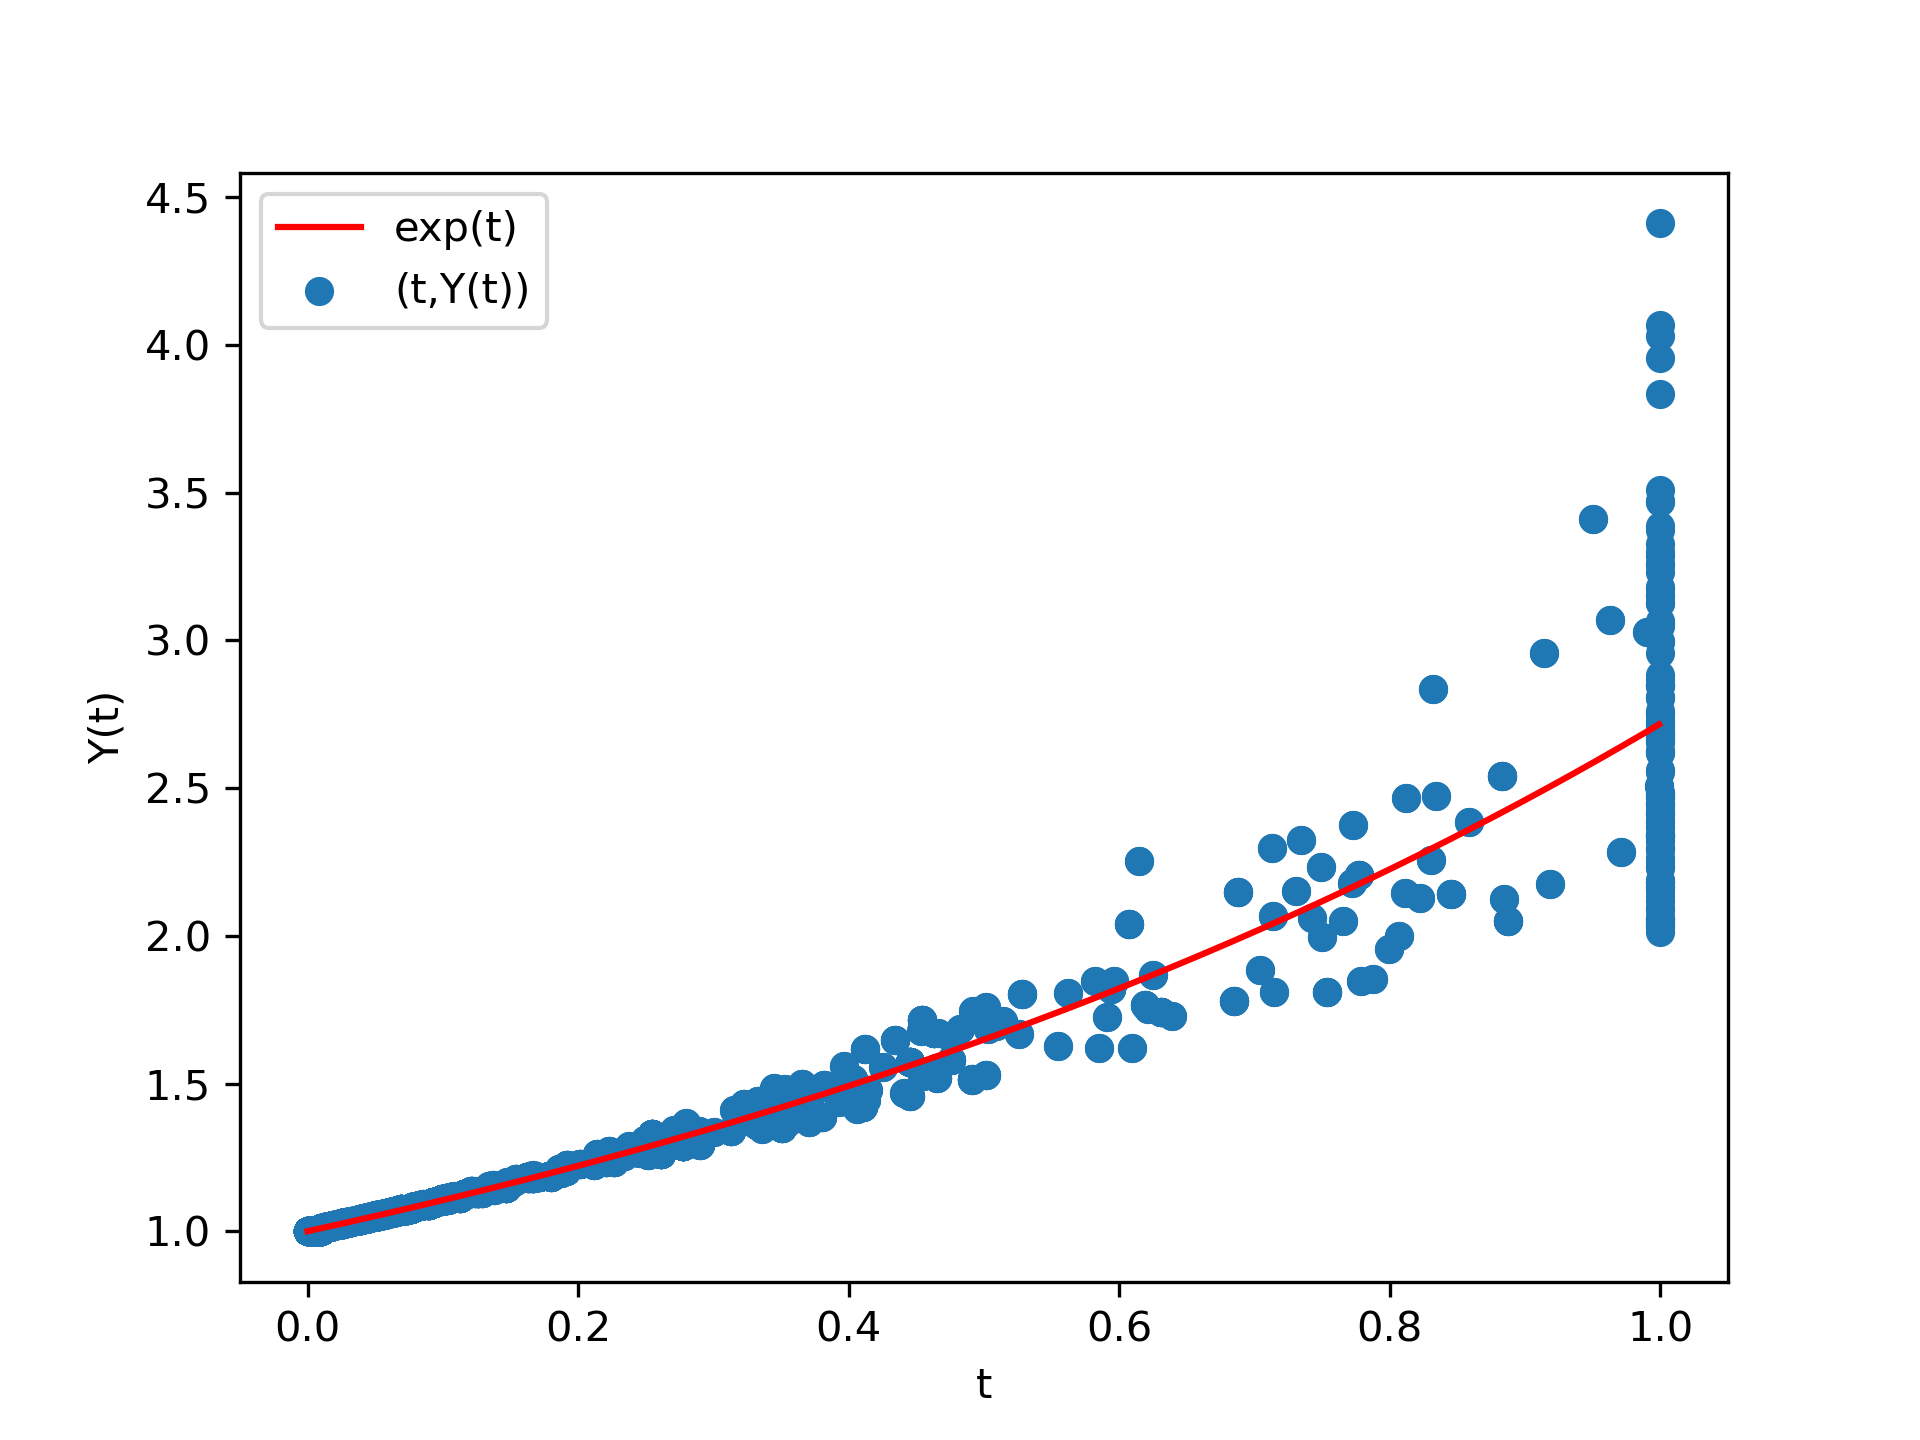
\includegraphics[width=0.8\textwidth]{plots/intro example.png}
        \caption{Recursive calls of code \ref{python eps ydy}}
        \label{fig:intro example}
    \end{figure}
\end{pythonn}

\subsection{Modifying Monte Carlo}

In this subsection, we discuss techniques for modifying RRVEs
in a way that preserves the expected value of the solution while
acquiring more desirable properties. These techniques are only
effective when applied smartly by using prior information
about the problem or computational costs. \\

We will frequently interchange RVs with the same expected values.
This is why we introduce the following notation.
\begin{notation}[$\cong$]
    \[
        X \cong Y \iff E[X]=E[Y]
        .\]
\end{notation}

Russian roulette is a MC technique commonly employed in rendering algorithms.
The concept behind Russian roulette is to replace a RV with a
less computationally expensive approximation sometimes.

\begin{definition}[Russian roulette] \label{Russian roulette}
    We define Russian roulette on $X$ with free parameters
    $Y_{1} \cong Y_{2}$, $p \in [0,1]$
    and $U$ independent of $Y_{1}$, $Y_{2}$, $X$
    as follows:

    \begin{equation}
        X \cong
        \begin{cases}
            \frac{1}{p}(X - (1-p)Y_{1}) & \text{ if } U < p \\
            Y_{2}                       & \text{ else }
        \end{cases}.
    \end{equation}
\end{definition}


\begin{notation}[$B(p)$]
    Often Russian roulette will be used with $Y_{1}= Y_{2}= 0$.
    In that case, we use Bernoulli variables to shorten notation.
    \begin{equation}
        B(p) \sim \text{Bernoulli}(p) =
        \begin{cases}
            1 & \text{ if } U<p \\
            0 & \text{ else }
        \end{cases} .
    \end{equation}
\end{notation}

\begin{example}[Russian roulette] \label{ex:simple russian roulette}
    Let us consider the estimation of $E[Z]$, where $Z$ is defined as follows:

    \begin{equation}
        Z = U + \frac{f(U)}{1000}.
    \end{equation}

    Here, $f:\mathbb{R} \rightarrow [0,1]$ is an expensive function to compute.
    Directly estimating $E[Z]$ would involve evaluating $f$ for each sample,
    which can be computationally costly. To address this, we can modify $Z$ to:

    \begin{equation}
        Z \cong U + B\left(\frac{1}{100}\right)\frac{f(U)}{10}.
    \end{equation}

    This requires calling $f$ on
    average once every $100$ samples. This significantly reduces the
    computational burden while increasing the variance slightly thereby increasing
    the MC efficiency.\\
\end{example}

\begin{related}[example \ref{ex:simple russian roulette}]
    In example \ref{ex:simple Russian roulette}, it is also
    possible to estimate the expectations of the $2$ terms
    of $Z$ separately. Given the variances and computational costs
    of both terms, you can calculate the asymptotically optimal division
    of samples for each term. However, this is no longer the case with RMC.
    In \cite{rath_ears_2022}, a method is presented to estimate the optimal
    Russian roulette/splitting factors for rendering.
\end{related}


\begin{example}[Russian roulette on (\ref{recursive RV})] \label{ex: russian roulette}
    To address the issue of indefinite recursion in
    (\ref{recursive RV}), Russian roulette can be employed
    by approximating the value of $Y$ near $t = 0$ with $1$
    sometimes. Specifically, we replace the coefficient $t$
    in front of the recursive term with $B(t)$ when $t < 1$.
    The modified recursive expression for $Y(t)$ becomes:

    \begin{equation}\label{eq:rr example}
        y(t) \cong Y(t) =
        \begin{cases}
            1 + B(t)Y(Ut) & \text{ if } t < 1 \\
            1 + tY(Ut)    & \text{ else}
        \end{cases}.
    \end{equation}
\end{example}

\vspace{0.2cm}

\begin{pythonn}[implementation of (\ref{eq:rr example})] \label{RRpython}
    \pythoncode{python code/RR_ydy.py}
    Interestingly, $\forall t \le 1:Y(t)$ is the number of recursion calls
    to sample $Y(t)$ such that the average number of recursion
    calls equals $e^{t}$.
    \begin{figure}[h!]
        \centering
        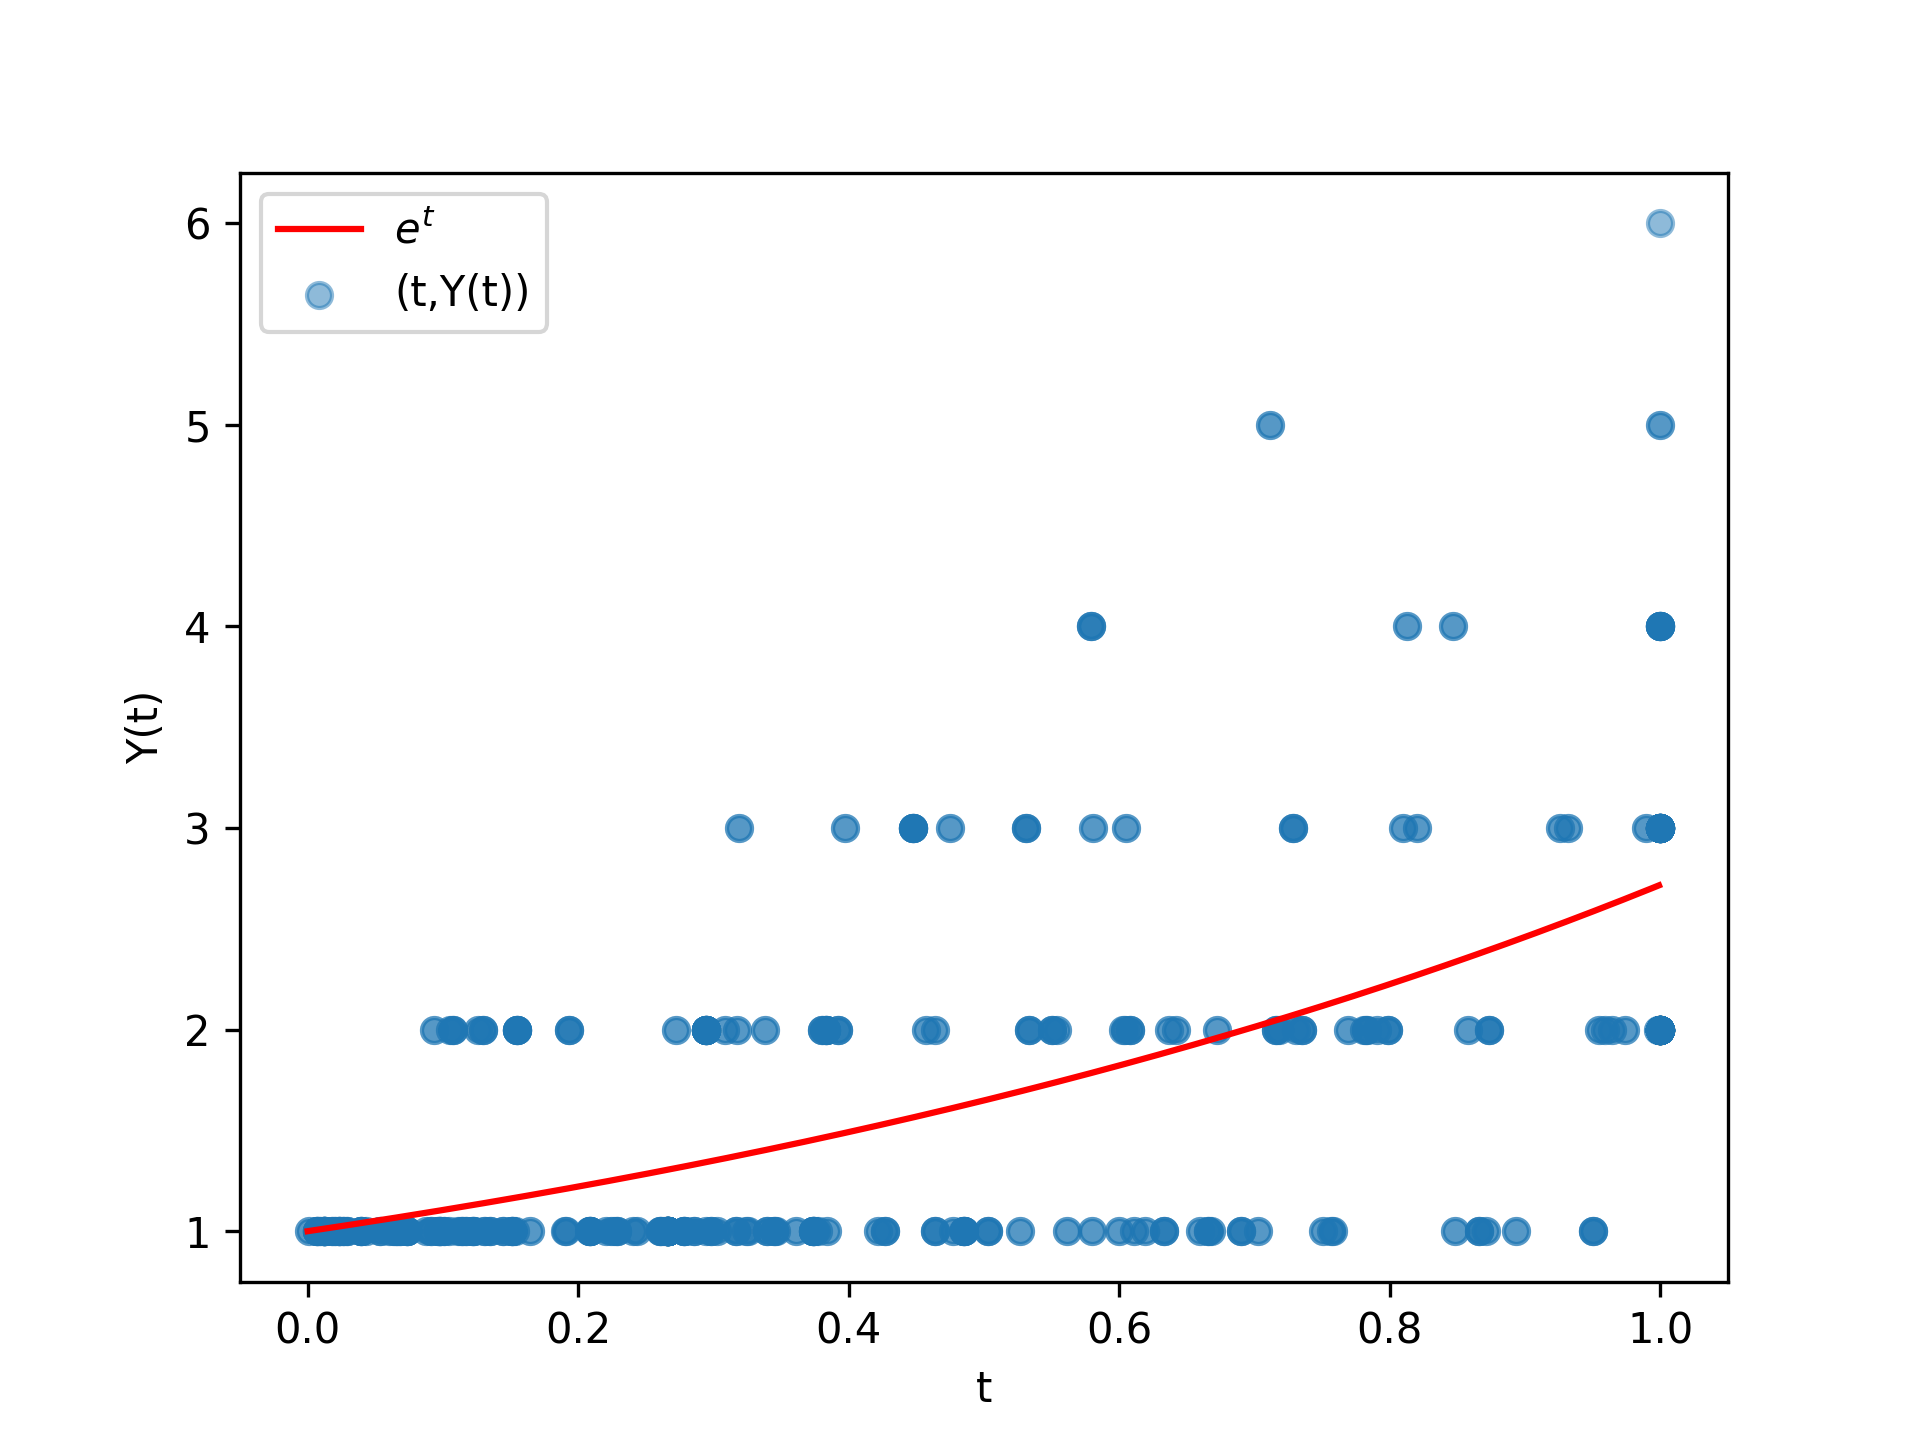
\includegraphics[width=0.8\textwidth]{plots/russian roulette example.png}
        \caption{Recursive calls $(t,Y(t))$ of code \ref{RRpython} }
        \label{fig:russian roulette}
    \end{figure}

\end{pythonn}

Splitting is a technique that has almost the reverse effect of Russian roulette.
Instead of reducing the number of simulations of a RV as Russian roulette does,
we increase it by using more samples (i.e. splitting the sample) which
reduces the variance.

\begin{definition}[splitting] \label{def:splitting}
    Splitting $X$ refers to utilizing multiple $X_{j} \sim X$ (not necessarily independent) to
    reduce variance by taking their average:
    \begin{equation}
        X \cong \frac{1}{N} \sum_{j=1}^{N} X_{j}.
    \end{equation}
\end{definition}

Splitting the recursive term in a RRVE can result in additive branching recursion,
necessitating cautious management of terminating the branches promptly to prevent
exponential growth in computational complexity. To accomplish this, termination
strategies that have been previously discussed can be employed. Subsequently,
we will explore the utilization of coupled recursion as a technique to mitigate
additive branching recursion in RRVEs (see example \ref{ex:coupled splitting}).

\begin{example}[splitting on (\ref{eq:rr example})] \label{ex:splitting}
    We can "split" the recursive term of (\ref{eq:rr example})
    into two parts as follows:

    \begin{equation}\label{eq:splitting}
        y(t) \cong Y(t) =
        \begin{cases}
            1 + \frac{B(t)}{2}(Y_{1}(Ut) + Y_{2}(Ut)) & \text{ if } t < 1 \\
            1 + \frac{t}{2}(Y_{1}(Ut) + Y_{2}(Ut))    & \text{ else}
        \end{cases}.
    \end{equation}

    where $Y_{1}(t)$ and $Y_{2}(t)$ are i.i.d. with $Y(t)$.
\end{example}

\vspace{0.2cm}

\begin{pythonn}[implementation of (\ref{eq:splitting})]
    \pythoncode{python code/SRR_ydy.py}
\end{pythonn}

\begin{definition}[control variates] \label{CV}
    Define control variating $f(X)$ with $\tilde{f}$ an approximation of $f$ as:
    \begin{equation}
        f(X) \cong f(X)-\tilde{f}(X) + E[\tilde{f}(X)].
    \end{equation}

    Note that control variating requires the evaluation of
    $E[\tilde{f}(X)]$. When this is estimated we refer to it as $2$-level MC.
\end{definition}


\begin{example}[control variate on (\ref{recursive RV})] \label{ex:CV}
    To create a control variate for (\ref{recursive RV}) that
    effectively reduces variance, we employ the approximation
    $y(t) \approx \tilde{y} =1+t$ and define the modified recursive term as follows:

    \begin{align}
        Y(t) & = 1 + E[\tilde{y}(Ut)] + t(Y(Ut) - \tilde{y}(Ut)) \\
             & = 1 + t + \frac{t^2}{2} + t(Y(Ut) - 1 - Ut).
    \end{align}

    Note that while we could cancel out the constant term
    of the control variate, doing so would have a negative impact
    on the Russian roulette implemented later.
\end{example}

\vspace*{0.2cm}
\begin{pythonn}[implementation of example \ref{ex:CV}]
    \pythoncode{python code/CVRR_ydy.py}
\end{pythonn}

\begin{related}[MC modification]
    For further reference on Russian roulette, splitting and control variates
    see \cite{veach_robust_1997}.
\end{related}

\subsection{Monte Carlo Trapezoidal Rule}

In this subsection, we introduce a MC trapezoidal rule that
exhibits similar convergence behavior to the methods discussed later.
The MC trapezoidal rule is essentially a regular Monte Carlo method
enhanced with control variates based on the trapezoidal rule.

\begin{definition}[MC trapezoidal rule]
    We define the MC trapezoidal rule for approximating the integral
    of function $f$ over the interval $[x, x+\Delta x]$ with a Russian roulette rate
    $l$ and $\tilde{f}$ the linear approximation of $f$ corresponding
    to the trapezoidal rule as follows:

    \begin{align}
         & \int_{x}^{x+\Delta x} f(s) ds                           \\
         & = \int_{x}^{x+\Delta x}  \tilde{f}(s) ds +
        \int_{x}^{x+\Delta x}  f(s) - \tilde{f}(s) ds              \\
         & = \Delta x \frac{f(x) + f(x+\Delta x)}{2}
        + E \left[f(S) - \tilde{f}(S)\right]                       \\
         & \cong \Delta x \frac{f(x) + f(x+\Delta x)}{2} \nonumber \\
         & + \Delta x l B\left( \frac{1}{l}\right)
        \left(f(S) - f(x) - \frac{S - x}{\Delta x}
        \left(f(x+\Delta x) - f(x)\right) \right), \label{eq:MCtrap}
    \end{align}

    where $S \sim \text{Uniform}(x,x+\Delta x)$.
\end{definition}

\begin{lemma}[RMSE MC Trapezoidal Rule] \label{lem:rmse mctrap}
    The MC trapezoidal rule
    for a twice differentiable function has
    \begin{equation}
        \text{RMSE} =O\left( \Delta x^{3} \right) .
    \end{equation}
\end{lemma}

\begin{proof}
    Start from (\ref{eq:MCtrap}). The MSE is the variance
    so we can ignore addition by constants.

    \begin{equation}
        \text{MSE} = \text{Var}\left( \Delta x l B\left( \frac{1}{l}\right)
        \left(f(S) - f(x) - \frac{S - x}{\Delta x}
        \left(f(x+\Delta x) - f(x)\right) \right)\right)
    \end{equation}
    We substitute $S = \Delta x U + x$ and then apply Taylor's theorem
    finishing the proof:

    \begin{align}
        \text{MSE} & = \text{Var}\left( \Delta x l B\left( \frac{1}{l}\right)
        \left(f(\Delta x U+x) - f(x) - U
        \left(f(x+\Delta x) - f(x)\right) \right)\right)                           \\
                   & = \text{Var}\left( \Delta x l B\left( \frac{1}{l}\right)
        \left( U \Delta x f'(x)+ \frac{U^{2} \Delta x ^{2}}{2} f''(Z_{1})
        - U \left( \Delta x f'(x) +
        \Delta x ^{2} f''(z_{2})\right) \right)\right)                             \\
                   & = \text{Var}\left( \Delta x l B\left( \frac{1}{l}\right)
        \left( \frac{U^{2} \Delta x ^{2}}{2} f''(Z_{1})
        -  \frac{U\Delta x ^{2}}{2} f''(z_{2}) \right)\right)                      \\
                   & =\Delta x ^{6} \text{Var}\left(  l B\left( \frac{1}{l}\right)
        \left( \frac{U^{2} }{2} f''(Z_{1})
        -  \frac{U}{2} f''(z_{2}) \right)\right),
    \end{align}
    for some $Z_{1} \in [x,S], z_{2} \in [x,x+\Delta x]$. The variance term is bounded
    because the variance of a bounded RV is bounded.
    Note that the proof doesn't rely on Russian roulette ($l=1$).
\end{proof}

\begin{related}[proof \ref{lem:rmse mctrap}]
    An easier to generalize proof to other types of control variates
    can be made by using ''separation of the main part''
    see lemma 4 of \cite{mathe_monte_nodate}.
\end{related}


\begin{definition}[composite MC trapezoidal rule] \label{MCtrap}
    Define the composite MC trapezoidal rule for approximating the integral
    of function $f$ over the interval $[a, b]$ with a uniform grid
    $(x_{j}) = \text{linspace}(a,b,n)$ with $n$
    intervals and a Russian roulette rate $l$ as follows:

    \begin{align} \label{eq:cMCtrap}
        \int_{a}^{b} f(s) ds \cong \Delta x \sum_{j=1}^{n} & \frac{f(x_{j}) + f(x_{j}+\Delta x)}{2} \nonumber \\
                                                           & + l B\left(\frac{1}{l}\right)
        \left(f(S_j) - f(x_{j}) - \frac{S_j - x_{j}}{\Delta x}(f(x_{j}+\Delta x) - f(x_{j}))\right),
    \end{align}

    where $S_j \sim \text{Uniform}(x,x+\Delta x)$.

\end{definition}

\begin{pythonn}[implementation of (\ref{eq:cMCtrap})]
    We implement (\ref{eq:cMCtrap}) for $\int_{0}^{1}e^{s}ds$.
    \vspace*{0.5cm}
    \pythoncode{python code/trap1.py}

    \begin{figure}[h!]
        \centering
        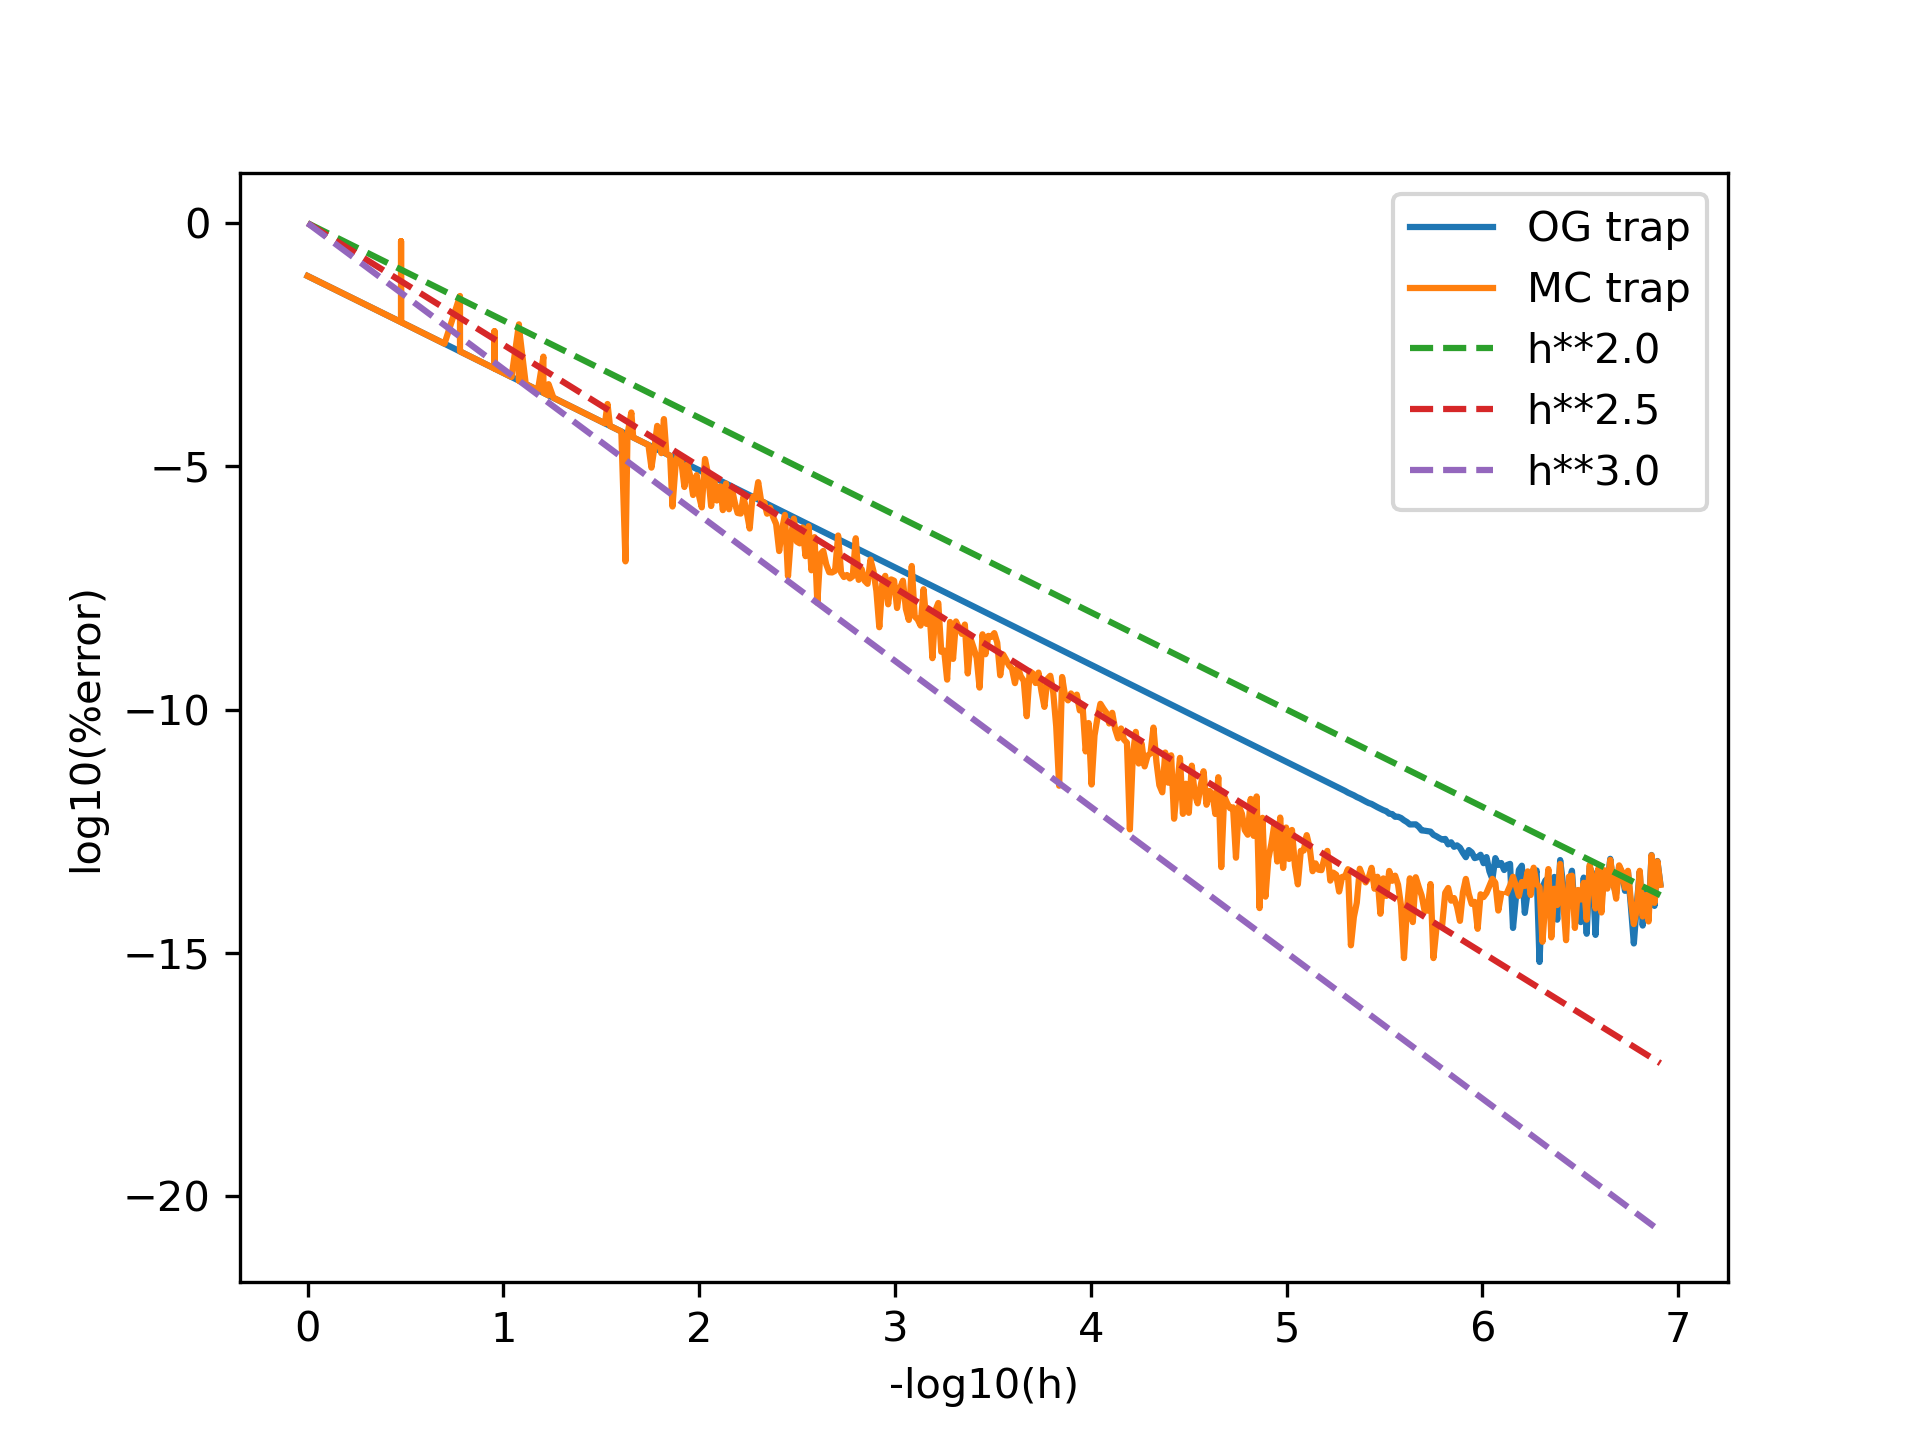
\includegraphics[width=0.8\textwidth]{plots/MCtrap.png}
        \caption{Log-log plot of the error of (\ref{eq:cMCtrap}) for
        $\int_{0}^{1}e^{s}ds$ with $l=100$. At floating point accuracy,
        the convergence ceases.
        }
        \label{fig:MCtrap}
    \end{figure}
\end{pythonn}

Figure \ref{fig:MCtrap} suggests that the order of convergence of RMSE of the
composite MC trapezoidal rule is better by $0.5$ than the normal composite trapezoidal rule.
The MC trapezoidal rule has on average $\frac{1}{l}$ more function calls than
the normal trapezoidal rule. For the composite rule with $n$ intervals,
there are $\text{Binomial}(n,\frac{1}{l})$ additional function calls
(repeated Bernoulli experiments). So they use up to a constant the same amount
of function calls on average. This means an advantage in IBC measured in RMSE. \\

\begin{theorem}[RMSE Composite Trapezoidal MC Rule] \label{thrm:order trap}
    The composite trapezoidal MC rule  wth $n$ intervals
    for a twice differentiable function has
    \begin{equation}
        \text{RMSE} =O\left(\frac{1}{n^{2.5}} \right) .
    \end{equation}

\end{theorem}

The proof uses lemma \ref{lem:rmse mctrap}
and is similar to the proof of the normal
trapezoidal rule with the main difference being  the
accumulation of ''local truncation'' errors into ''global truncation'' error.
Normally there is a loss of one order but the MC trapezoidal loses only a half order
because the accumulation happens in variance instead of bias.

\begin{align}
    \sqrt{\text{Var}\left(\sum_{j=1}^{n}  \Delta x^{3}U_{j}^{2}\right)}
     & = \Delta x^{3} \sqrt{ \sum_{j=1}^{n}\text{Var} (U_{j}^{2})} \\
     & = \Delta x^{3} \sqrt{ n \text{Var}(U^{2})}                  \\
     & = O( \Delta x^{2.5}).
\end{align}

Note that the meaning of a bound on the error that behaves as $O(\Delta x^{2})$ and
a bound on the RMSE that behaves as $O(\Delta x^{2})$ is different.
A bound on the error implies a bound on the RMSE, but
the reverse is not true.

\begin{related}[Monte Carlo Trapezoidal Rule]
    With Stein's paradox, it is always possible to bias the composite MC trapezoidal
    rule to achieve lower RMSE.
    The optimal IBC for the deterministic, random and quantum case
    are known see \cite{heinrich_optimal_2001} for some smoothness classes.
\end{related}


\subsection{Unbiased Non-Linearity}

In this subsection, we present techniques for handling polynomial non-linearity.
The backbone for this is using independent samples
$y^{2} \cong Y_{1} Y_{2}$ with $Y_{1}$ independent of $ Y_{2}$ and
$Y_{1} \cong Y_{2} \cong y$.


\begin{example}[$y_t=y^{2}$] \label{ex:nonlinear example}
    Consider the following ODE:

    \begin{equation} \label{eq:nonlinear example}
        y_t = y^2, \quad y(1) = -1.
    \end{equation}

    The solution to this equation is given by $y(t) = -\frac{1}{t}$.
    By integrating both sides of (\ref{eq:nonlinear example}),
    we obtain the following integral equation:

    \begin{equation}
        y(t) = -1 + \int_{1}^{t} y(s) y(s)ds.
    \end{equation}

    To estimate the recursive integral in (\ref{eq:nonlinear example}),
    we use i.i.d. $Y_1,Y_2 \sim Y$ in following RRVE:

    \begin{equation} \label{RRVE: nonlinear example}
        y(t) \cong Y(t) = -1 + (t-1) Y_1(S) Y_2(S),
    \end{equation}

    where $S \sim \text{Uniform}(1,t)$.
    Branching RRVEs are typical when dealing
    with non-linearity.
\end{example}

\vspace*{0.2cm}
\begin{pythonn}[implementation of example \ref{ex:nonlinear example}]\label{py:nonlinear example}
    \pythoncode{python code/dyy2.py}
    In this implementation $Y(t)$ only takes values $\{-1,0\}$.
\end{pythonn}

\begin{example}[$e^{E[X]}$] \label{ex:exp int}
    $e^{\int x(s)ds}$ is a common expression encountered when studying ODEs.
    In this example, we demonstrate how you can generate unbiased estimates of
    $e^{E[X]}$ with simulations of $X$. The Taylor series of $e^{x}$ is:
    \begin{align}
        e^{E[X]} & = \sum_{n=0}^{\infty} \frac{E^{n}[X]}{n!}     \\
                 & = 1 + \frac{1}{1}E[X]\left(1+ \frac{1}{2}E[X]
        \left(1+\frac{1}{3}E[X]\left(1+ ...\right)\right)\right). \label{taylor e}
    \end{align}
    Change the fractions of (\ref{taylor e}) to Bernoulli processes
    and replace all $X$ with independent $X_j \cong X$.
    \begin{align}
        e^{E[X]} & = E
        \left[1 + B\left(\frac{1}{1}\right)E[X_1]
        \left(1+ B\left(\frac{1}{2}\right)E[X_2]
        \left(1+B\left(\frac{1}{3}\right)E[X_3]
        \left(1+ ...\right)
        \right)
        \right)
        \right]                             \\
                 & \cong \label{eq:exp int}
        1 + B\left(\frac{1}{1}\right)X_1
        \left(1+ B\left(\frac{1}{2}\right)X_2
        \left(1+B\left(\frac{1}{3}\right)X_3
            \left(1+ ...\right)
            \right)
        \right).
    \end{align}
    Sampling (\ref{eq:exp int}) requires a finite amount of samples from $X_{j}$'s
    with probability $1$.
\end{example}

\begin{related}[example \ref{ex:exp int}]
    NVIDIA has a great paper on optimizing example \ref{ex:exp int}
    \cite{kettunen_unbiased_2021}.
\end{related}

\subsection{Recursion}

In this subsection, we discuss recursion-related techniques.

\begin{technique}[coupled recursion]
    The idea behind coupled recursion is sharing recursion calls of
    multiple RRVEs for simulation. This does make them dependent.
\end{technique}

\begin{example}[coupled recursion] \label{ex:coupled recursion}
    Consider calculating the
    sensitivity of following ODE to a
    parameter $a$:
    \begin{align}
        y_t             & =ay,y(0)=1 \Rightarrow \label{couple recu ex1} \\
        \partial_{a}y_t & = y + a \partial_{a}y \label{couple recu ex2}
    \end{align}
    Turn (\ref{couple recu ex1}) and (\ref{couple recu ex2}) into RRVEs.
    To emphasize that they are coupled, that they should
    recurse together we write them in a matrix equation:
    \begin{equation} \label{coupled mat}
        \begin{bmatrix}
            y(t) \\
            \partial_{a}y(t)
        \end{bmatrix} \cong
        \begin{bmatrix}
            Y(t) \\
            \partial_{a}Y(t)
        \end{bmatrix}=
        X(t)=
        \begin{bmatrix}
            1 \\
            0
        \end{bmatrix}+
        t \begin{bmatrix}
            a & 0 \\
            1 & a
        \end{bmatrix}
        X(Ut).
    \end{equation}

    Observe how this eliminates the additive branching recursion
    present in (\ref{couple recu ex2}).

\end{example}

\begin{pythonn} [implementation of (\ref{coupled mat})]
    \pythoncode{python code/coupled_mat.py}
\end{pythonn}

\begin{related}[coupled recursion]
    Example \ref{ex:coupled recursion} is inspired by \cite{vicini_path_2021}.
    \cite{vicini_path_2021} propose an efficient unbiased backpropagation
    algorithm for rendering.
\end{related}

\begin{technique}[recursion in recursion]\label{tech:recu in recu}
    Recursion in recursion is like proving an induction
    step of an induction proof with induction. Recursion in recursion
    uses an inner recursion in the outer recursion.
\end{technique}

\begin{related}[recursion in recursion]
    Beautiful examples of recursion in recursion are
    the next flight variant of WoS in
    \cite{sawhney_grid-free_2022} and epoch-based algorithms in optimization
    \cite{gupta_convergence_2021}.
\end{related}

Most programming languages do support recursion, but it often comes with certain
limitations such as maximum recursion depth and potential performance issues.
There are multiple ways to implement recursion we will discuss tail recursion and
do an example using a stack.

\begin{technique}[non-branching tail recursion]
    Tail recursion involves reordering all operations
    so that almost no operation needs to happen after
    the recursion call. This allows us to return the
    answer without retracing all steps when we reach
    the last recursion call and it can achieve similar
    speeds to a forward implementation.
\end{technique}

The non-branching recursion presented in the RRVEs
can be implemented with tail recursion due to the associativity of
all operations ($(xy)z = x(yz)$) involved.

\begin{pythonn}[tail recursion on (\ref{coupled mat})] \label{py:tail recursion couple}
    We implement (\ref{coupled mat}) but this time with tail recursion.
    We collect addition operations in a vector $sol$ and multiplication
    in a matrix $W$. $W$ may be referred to as accumulated weight or throughput.
    \vspace{0.3cm}
    \pythoncode{python code/tailrecu.py}
\end{pythonn}

Tail recursion is not always desirable as it discards intermediate values of
the recursion calls and can increase
computational cost.
To retain some of these intermediate values, it is possible to use tail recursion partially.
In example \ref{py:tail recursion couple} it would
be more efficient to avoid matrix multiplication on line $7$. An alternative
to tail recursion is implementing the recursion with a stack.

\begin{pythonn}[stack recursion on (\ref{coupled mat})] \label{py:stack recursion couple}
    We implement (\ref{coupled mat}) but this time with a stack.
    We want to avoid matrix multiplication and only use matrix-vector multiplications.
    To do this on (\ref{coupled mat}) we need to know $X(Ut)$ when
    it doesn't get Russian rouletted away. If we sample $Ut$ we can recurse
    on our reasoning until Russian roulette termination so we need the path
    of all the samples.
    \vspace{0.3cm}
    \pythoncode{python code/stackrecu.py}
\end{pythonn}


\section{Ordinary Differential Equations}

\subsection{Green's Functions}
In this subsection, we discuss how to turn ODEs into integral equations and
then solving them. Our main tool for this is Green's functions. \\

Roughly speaking Green's functions are a type
of kernel function used to solve linear problems with linear
conditions (it is also possible to absorb less important non-linear terms in
the source term). In this context the Green's functions are
like homogenous and particular solutions to a specific problem
that are combined with integration to solve more general problems.

\begin{related}[Green's function]
    Our notion of Green's function is similar
    to that in \cite{hwang_simulationtabulation_2001}.
\end{related}


\begin{notation}[$H$]
    We denote the Heaviside step function with:
    \begin{equation}
        H(x) = \begin{cases}
            0 & \text{ if } x<0 \\
            1 & \text{ else }
        \end{cases}.
    \end{equation}
\end{notation}

\begin{notation}[$\delta$]
    We denote the Dirac delta function with $\delta(x)$.
\end{notation}


To clarify Green's functions let's look at the following example.

\begin{example}[$y_t=y$ average condition]
    We will solve the equation:

    \begin{equation} \label{ydy int}
        y_t = y,
    \end{equation}

    but this time with a different condition:

    \begin{equation}
        \int_{0}^{1} y(s) ds = e-1.
    \end{equation}

    The solution to this equation remains the same: $y(t) = e^{t}$.
    We define the corresponding source Green's function $G(t,x)$ for $y_t$
    and this type of condition as follows:

    \begin{equation}
        G_t = \delta(x-t), \quad \int_{0}^{1} G(s,x) ds = 0.
    \end{equation}

    Solving this equation yields:

    \begin{equation}
        G(t,x) = H(t-x) + x - 1.
    \end{equation}

    We define the corresponding boundary Green's function $G(t,x)$ for $y_t$
    and this type of condition as follows:

    \begin{equation}
        P_{t} = 0, \quad \int_{0}^{1} P(s) ds = e -1.
    \end{equation}

    Solving this equation yields:

    \begin{equation}
        P(t) = e -1.
    \end{equation}

    The Green's functions are constructed such that
    we can form the following integral equation for (\ref{ydy int}):

    \begin{equation} \label{int ydy int}
        y(t) = P(t) + \int_{0}^{1} G(t,s) y(s) ds.
    \end{equation}

    Converting (\ref{int ydy int}) into a RRVE
    using RMC, we obtain:

    \begin{equation}\label{RRVE ydy int}
        Y(t) = e - 1 + 2B\left(\frac{1}{2}\right)Y(S)(H(t-S)+S-1),
    \end{equation}

    where $S \sim U$. We plot realizations of
    (\ref{RRVE ydy int}) in Figure \ref{fig:ydy int}.

    \begin{figure}[h!]
        \centering
        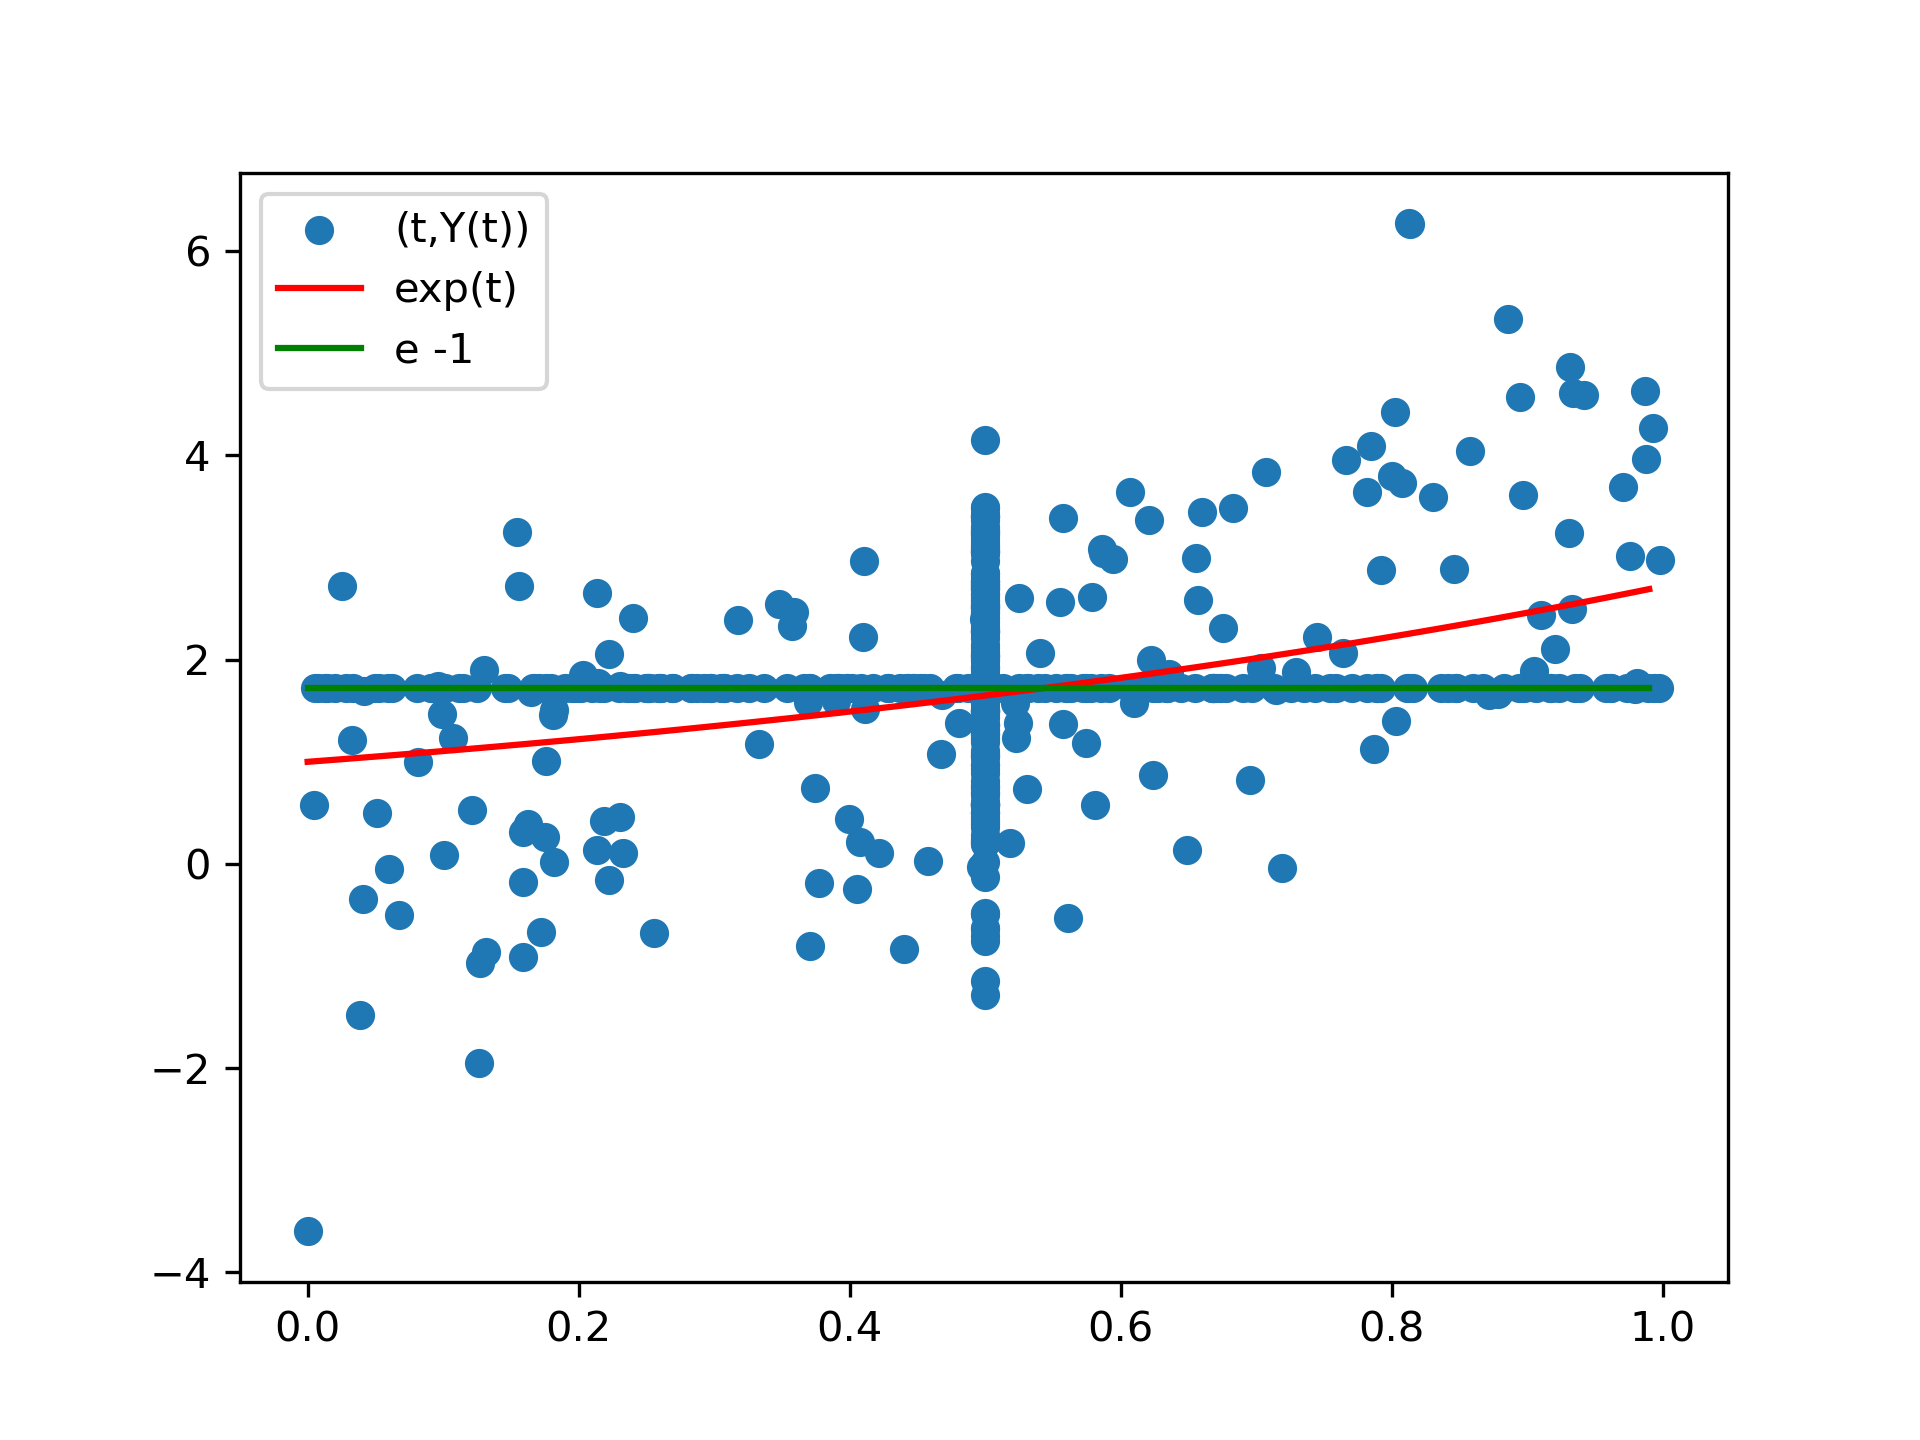
\includegraphics[width=0.8\textwidth]{plots/ydy int.png}
        \caption{Recursive calls $(t,Y(t))$ of (\ref{RRVE ydy int}) when
            calling $Y(0.5)$ $300$ times. Points accumulate on
            the Green's line due to the Russian roulette,
            and at  $t=0.5$ because it is the starting
            value of the simulation.
        }
        \label{fig:ydy int}
    \end{figure}

\end{example}

(\ref{int ydy int}) is a Fredholm integral
equations of the second kind.

\begin{definition}[Fredholm equation of the second kind]
    A Fredholm equation of the second kind for $\varphi$  is of the following form:
    \begin{equation}
        \varphi(t)=f(t)+\lambda \int_a^b K(t, s) \varphi(s) ds.
    \end{equation}
    Given the kernel  $K(t, s)$  and  $ f(t)$.
\end{definition}

If both $K$ and $f$ satisfy certain regularity conditions, then for sufficiently
small $\lambda$, it is relatively straightforward to establish the existence
and uniqueness of solutions using a fixed-point argument.

\begin{example}[Dirichlet $y_{tt}=y$] \label{main dirichlet}
    We turn the following ODE into Fredholm integral equation of
    the second kind for testing:
    \begin{equation} \label{eq:main dirichlet}
        y_{tt}=y, \quad y(b_{0}),y(b_{1}).
    \end{equation}
    The Green's functions corresponding to $y_{tt}$ and Dirichlet conditions are:

    \begin{align}
        P(t,x) & = \begin{cases}
                       \frac{b_{1}-t}{b_{1}-b_{0}} & \text{if } x = b_{0} \\
                       \frac{t-b_{0}}{b_{1}-b_{0}} & \text{if } x = b_{1}
                   \end{cases},       \\
        G(t,s) & = \begin{cases}
                       -\frac{(b_{1}-t)(s-b_{0})}{b_{1}-b_{0}} & \text{if } s<t \\
                       -\frac{(b_{1}-s)(t-b_{0})}{b_{1}-b_{0}} & \text{if } t<s
                   \end{cases}.
    \end{align}
    Straight from these Green's functions, you get the following integral equation and RRVE:
    \begin{align} \label{inteq:main dirichlet}
        y(t) & = P(t,b_{0}) y(b_{0}) + P(t,b_{1}) y(b_{1}) +
        \int_{b_{0}}^{b_{1}} G(t,s)y(s) ds,                  \\
        Y(t) & = P(t,b_{0}) y(b_{0}) + P(t,b_{1}) y(b_{1})
        + l B\left(\frac{1}{l} \right)(b_{1}-b_{0}) G(t,S)y(S) , \label{RRVE:main dirichlet}
    \end{align}
    where $l \in \mathbb{R}$ the Russian roulette rate is and
    $S \sim \text{Uniform}(b_{1},b_{0})$. In Figure \ref{fig:mainD explosion}
    we tested convergence of (\ref{RRVE:main dirichlet}).

\end{example}

\begin{figure}[h!]
    \centering
    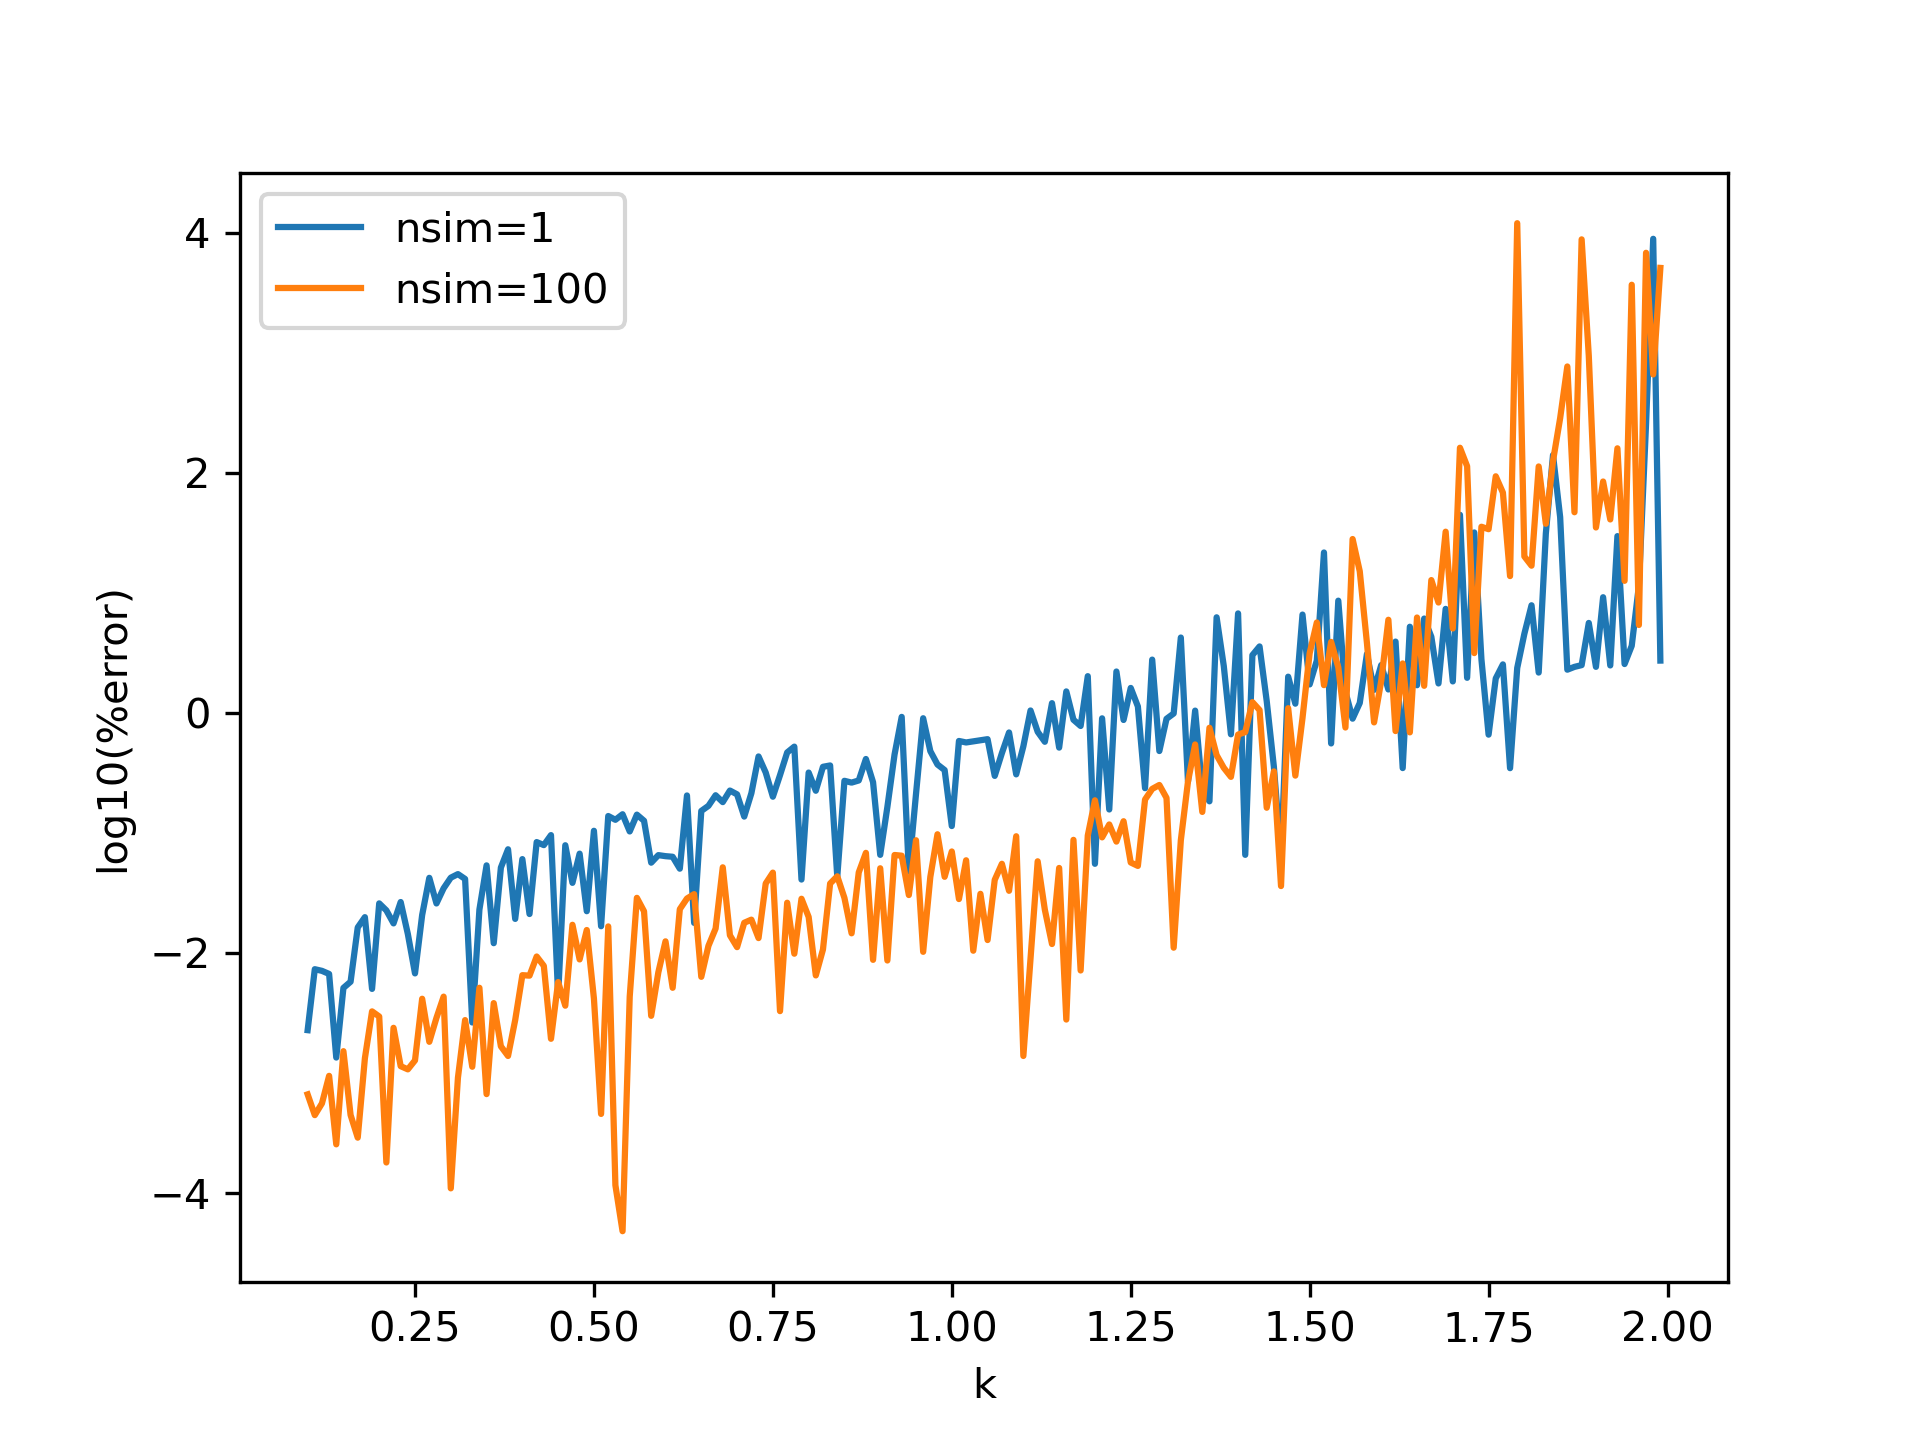
\includegraphics[width=0.8\textwidth]{plots/mainD explosion.png}
    \caption{The logarithmic percentage error of $Y(0)$ for
    (\ref{RRVE:main dirichlet}), with $l=1.2$ and initial conditions
    $y(-k)=e^{-k}$ and $y(k)=e^{k}$, displays an exponential
    increase until approximately $k=1.5$, beyond which additional
    simulations fail to reduce the error, indicating that the variance
    doesn't exist.}
    \label{fig:mainD explosion}
\end{figure}

Coupled splitting is one of the ideas that we tested on example \ref{main dirichlet}.
Coupled splitting deals with additive branching of splitting by coupling (reusing)
samples.

\begin{example}[coupled splitting on example \ref{main dirichlet}] \label{ex:coupled splitting}
    In addition to normal splitting (see definition \ref{def:splitting}),
    we can also split the domain in (\ref{inteq:main dirichlet})
    as follows:

    \begin{align}\label{inteq:coupled splitting}
        y(t) & = P(t,b_{0}) y(b_{0}) + P(t,b_{1}) y(b_{1}) +
        \frac{1}{2} \int_{b_{0}}^{b_{1}} G(t,s)y(s) ds +
        \frac{1}{2} \int_{b_{0}}^{b_{1}} G(t,s)y(s) ds,                                             \\
        y(t) & = P(t,b_{0}) y(b_{0}) + P(t,b_{1}) y(b_{1}) + \label{inteq:coupled domain splitting}
        \int_{b_{0}}^{\frac{b_{1}+b_{0}}{2}} G(t,s)y(s) ds +
        \int_{\frac{b_{1}+b_{0}}{2}}^{b_{1}} G(t,s)y(s) ds.
    \end{align}

    By coupling, we can eliminate the additive branching recursion
    in the RRVEs corresponding to (\ref{inteq:coupled splitting})
    and (\ref{inteq:coupled domain splitting}).
    This results in the following RRVE:

    \begin{equation} \label{RRVE:coupled splitting}
        X(t_{1},t_{2})=
        \begin{bmatrix}
            P(t_{1},b_{0}) & P(t_{1},b_{1}) \\
            P(t_{2},b_{0}) & P(t_{2},b_{1})
        \end{bmatrix}
        \begin{bmatrix}
            y(b_{0}) \\
            y(b_{1})
        \end{bmatrix}
        +
        W
        \begin{bmatrix}
            G(t_{1},S_{1}) & G(t_{1},S_{2}) \\
            G(t_{2},S_{1}) & G(t_{2},S_{2})
        \end{bmatrix}
        X(S_{1},S_{2}),
    \end{equation}
    where $W$ the right weighting matrix is
    (see code \ref{py:coupled splitting}),
    $S_{1}$ and $S_{2}$ can be chosen
    in various ways. (\ref{RRVE:coupled splitting}) is unbiased in the following way:
    $X(t_{1},t_{2}) \cong [y(t_{1}) \quad y(t_{2})]^{T}$.

\end{example}

\begin{pythonn}[implementation of (\ref{RRVE:coupled splitting})] \label{py:coupled splitting}
    We implemented (\ref{RRVE:coupled splitting}) with recursion but in this case, it
    is better to implement it forwardly. \\
    \pythoncode{python code/coupled_splitting.py}

    \begin{figure}[h!]
        \centering
        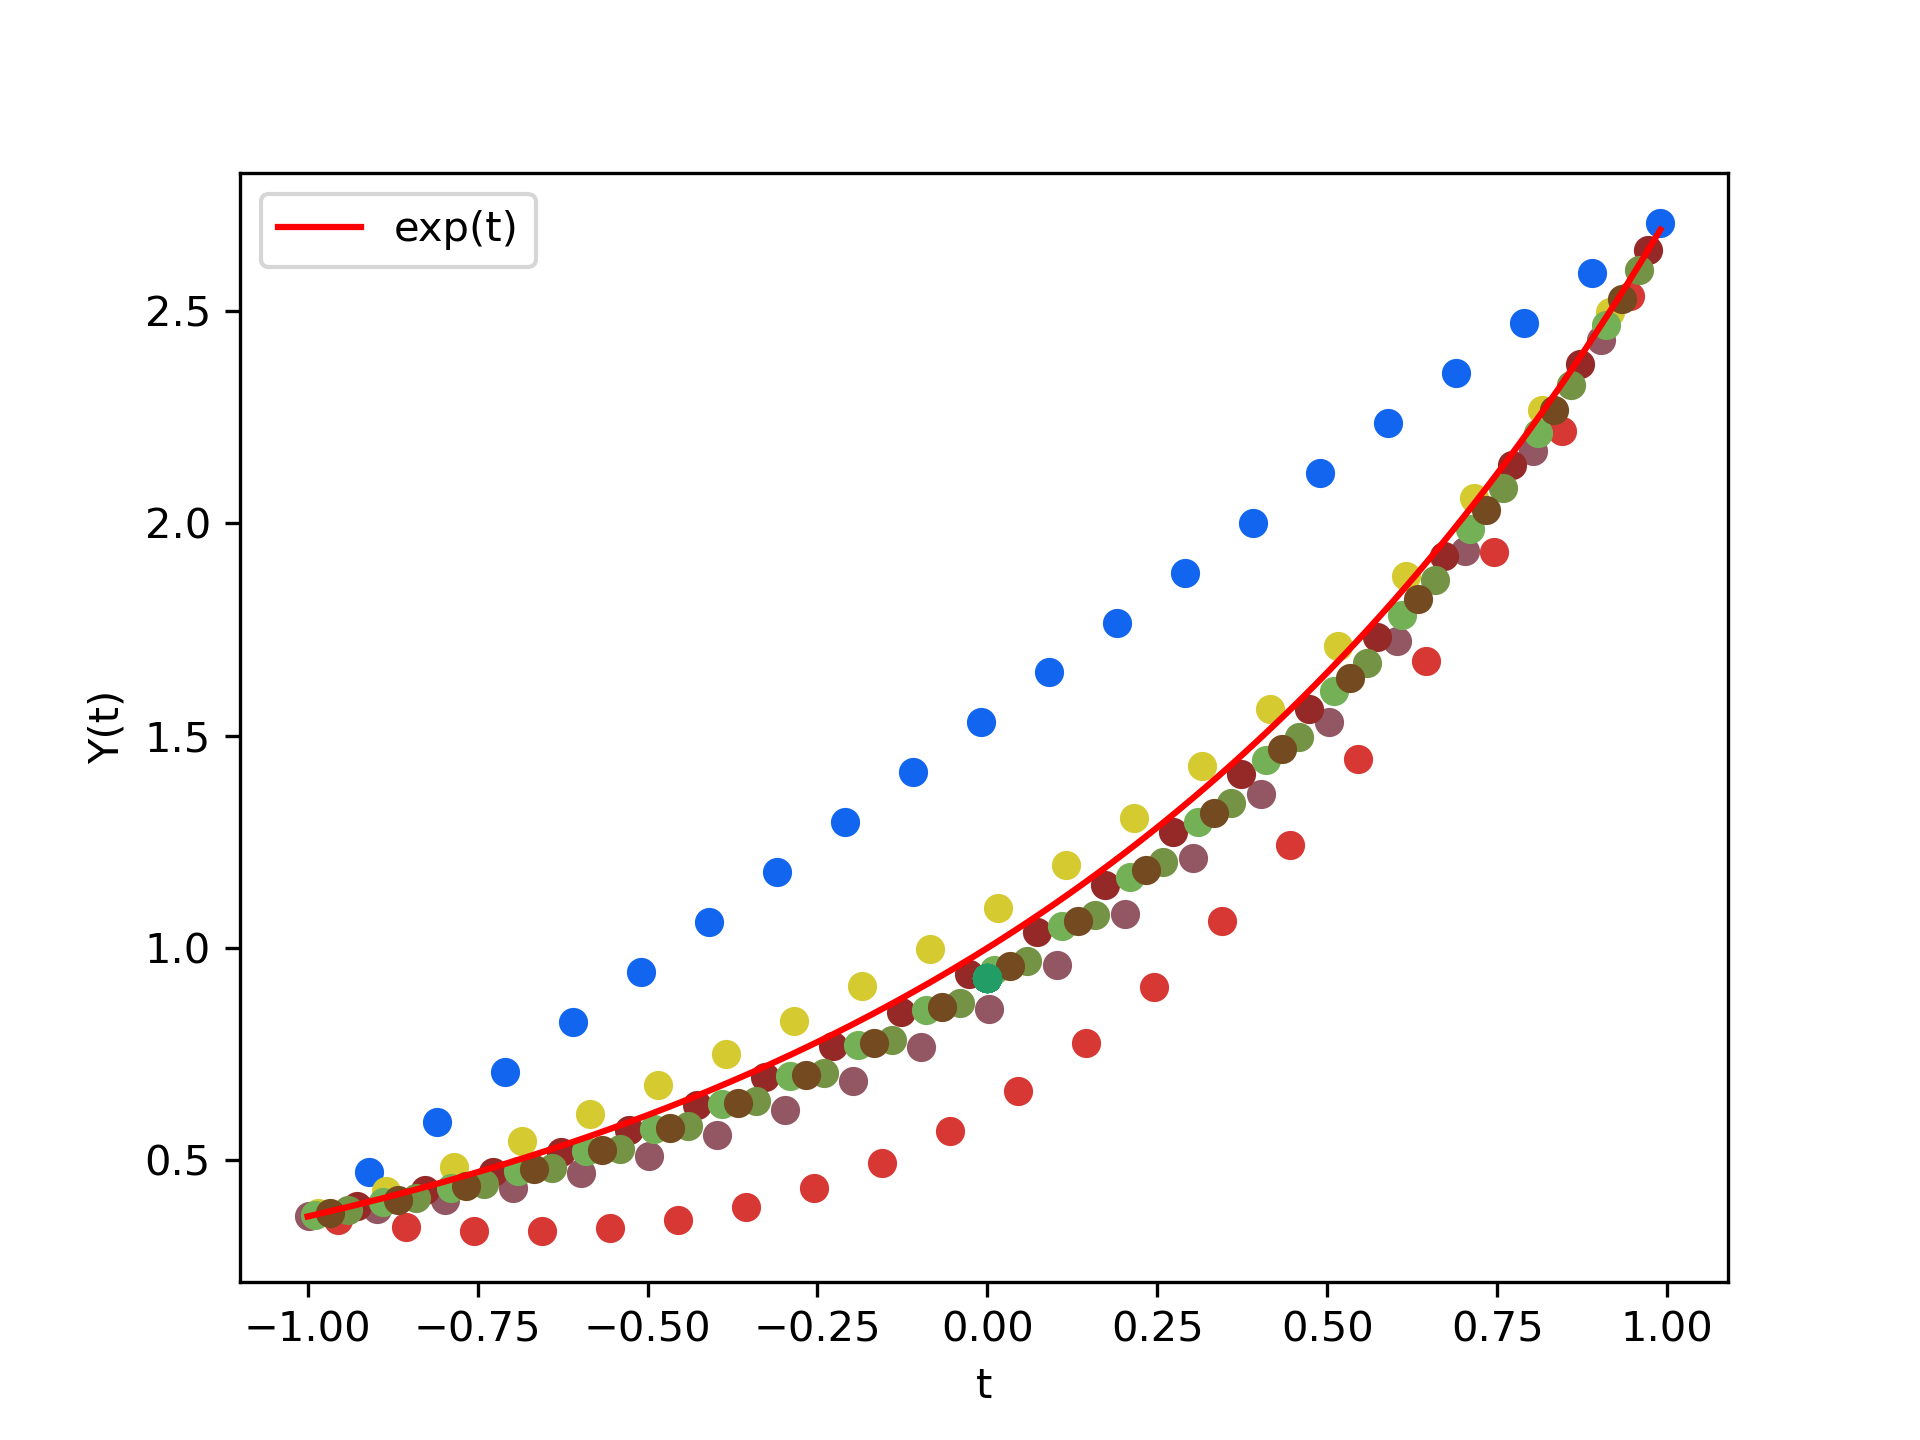
\includegraphics[width=0.8\textwidth]{plots/coupled split.png}
        \caption{Recursive calls of (\ref{RRVE:coupled splitting}) when
        calling $X(0)$ once. We chose $X$ to have $20$ points and
        colored each call. The $S_{j}$ are coupled such that
        they are equally spaced.
        The initial conditions for this call are $y(-1)=e^{-1}$ and $y(1)=e^{1}$,
        with Russian roulette rate $l=1.2$. }
        \label{fig:coupled splitting}
    \end{figure}
\end{pythonn}

\begin{related}[coupled splitting]
    Coupled splitting is partly inspired by how \cite{sabelfeld_sparsified_2009}
    reduces variance by using bigger submatrices.
    Reusing samples for WoS is discussed
    in \cite{miller_boundary_2023} and \cite{bakbouk_mean_2023}.
\end{related}

Figure \ref{fig:coupled splitting}
resembles fixed-point iterations, leading us to hypothesize
that the convergence
speed is very similar to fix-points methods until the accuracy
of the stochastic approximation of the operator is reached
(the approximate operator bottleneck). The approximation of the operator
can be improved by increasing the coupled splitting amount when
approaching the bottleneck. Alternatively when reaching
the bottleneck it is possible to rely on MC convergence.

\begin{related}[convergence coupled splitting]
    See \cite{gupta_convergence_2021} for a discussion on the convergence
    of recursive stochastic algorithms.
\end{related}


\begin{related}[IBC integral equations]
    Optimal IBC is known for integral equations see \cite{heinrich_monte_nodate}
    for the solution in $1$ point and the global solution.
\end{related}

\subsection{Initial Value Problems}
Classic IVP solvers rely on shrinking the time steps for
convergence. In this subsection, we introduce
Recursion in Recursion MC (RRMC) for IVPs that tries to emulate
this behavior.


\begin{example}[RRMC $y_t=y$] \label{ex:RRMC IVP}
    We demonstrate RRMC for IVPs with

    \begin{equation}
        y_t = y, \quad y(0) = 1.
    \end{equation}

    Imagine we have a time-stepping scheme $(t_{n}), \forall n: t_{n-1} < t_{n}$
    then the following integral equations hold:

    \begin{equation}
        y(t)= y(t_{n}) + \int_{t_{n}}^{t}y(s)ds , \quad t>t_{n}.
    \end{equation}

    Turn these in the following class of RRVEs:

    \begin{equation}
        y(t) \cong Y_{j}(t) = y(t_{j}) + (t-t_{j})Y_{j}((t-t_{j})U+t_{j}), \quad t>t_{j}.
    \end{equation}

    A problem with these RRVEs is that we do not know $y(t_{j})$.
    Instead, we can replace it with an unbiased estimate $y_{j}$
    which we keep frozen in the inner recursion:
    \begin{align}
        \label{eq:RRMC IVP inner}
        y(t) \cong Y_{j}(t)  & = y_{j} + (t-t_{j})Y_{j}((t-t_{j})U+t_{j}), \quad t>t_{j} \\
        y(t_{j}) \cong y_{j} & = \begin{cases}
                                     Y_{j-1}(t_{j}) & \text{ if } j \neq 0 \\
                                     y(t_{0})       & \text{ if } j = 0
                                 \end{cases}.
        \label{eq:RRMC IVP outer}
    \end{align}
    We refer to (\ref{eq:RRMC IVP inner}) as the inner recursion and
    (\ref{eq:RRMC IVP outer}) as the outer recursion of the recursion in
    recursion.
\end{example}

\begin{pythonn}[implementation of example \ref{ex:RRMC IVP}] \label{py:RRMC IVP}
    \pythoncode{python code/RRMC_IVP.py}

    \begin{figure}[h!]
        \centering
        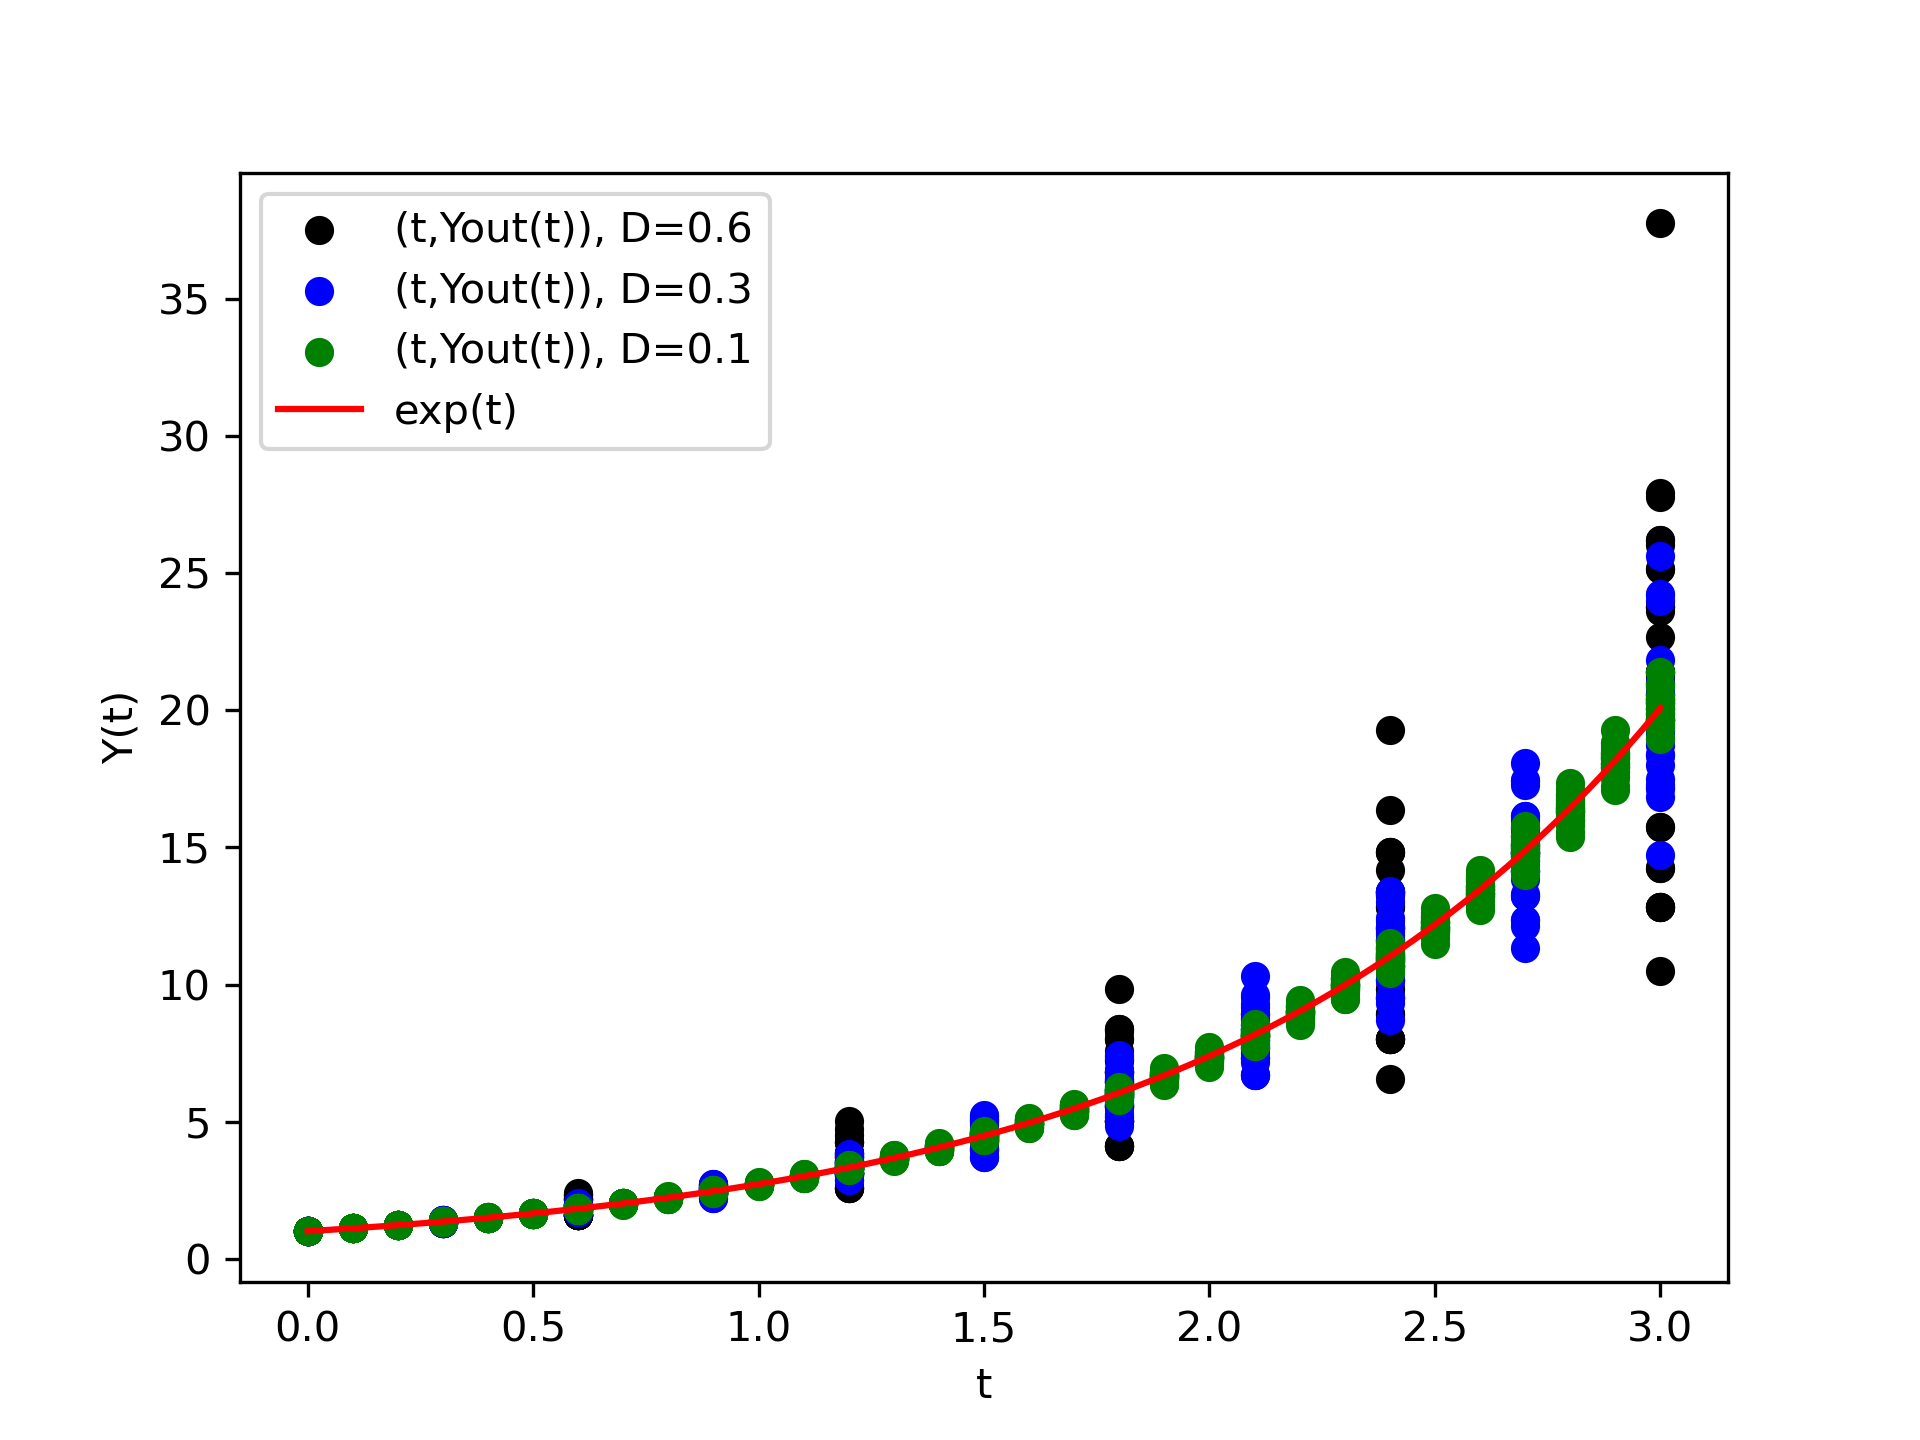
\includegraphics[width=0.8\textwidth]{plots/RRMC IVP.png}
        \caption{Recursive calls of (\ref{eq:RRMC IVP outer})
            when calling $Y_{\text{out}}(3,h)$ $30$ times for different $h$.  }
        \label{fig:RRMC IVP}
    \end{figure}
\end{pythonn}

We measured the convergence speed in RMSE of $Y(t)$ estimating $y(t)$  of example
\ref{ex:RRMC IVP} to be $O\left(h^{1.5} \right)$ with $h$ the step size.
We used a scaled version of the time process of example \ref{ex: russian roulette}
for the inner recursion such that the average amount of total inner recursion calls
is $e n$ with $n$ the total amount of outer recursion calls.
Our intuition for this behavior is based on how classical solvers
work and the MC trapezoidal rule.

\begin{conjecture}[local RMSE RMC]
    Consider a general linear IVP
    \begin{equation}
        y_{t}(t)= A(t)y(t)+g(t), y(t_{0}),
    \end{equation}
    with $A$ a matrix and $g$ a vector function each
    once differentiable with the corresponding RRVE
    \begin{equation}
        y(t) \cong Y(t) = y(t_{0}) + h B \left( \frac{t-t_{0}}{h}\right)
        A(S) Y(S) + g(S),
    \end{equation}
    with $S \sim \text{Uniform}(t_{0},t)$ there holds
    \begin{equation}
        E[||y(t_{1})-Y(t_{1})||^{2}] = O(h^{2}),
    \end{equation}
    with $t_{1} = t_{0} + h$.
\end{conjecture}


We can improve RRMC with control variates.
\begin{example}[CV RRMC $y_t=y$]\label{ex:CV RRMC IVP}
    Let us control variate example \ref{ex:RRMC IVP}.

    \begin{equation}
        y(t)= y(t_{n}) + \int_{t_{n}}^{t}y(s)ds , \quad t>t_{n}.
    \end{equation}

    We build a control variate with a lower-order approximation
    of the integrand:

    \begin{align}
        y(s) & = y(t_{n}) + (s-t_{n})y_t(t_{n}) + O((s-t_{n})^{2})      \\
             & \approx y(t_{n}) + (s-t_{n})f(y(t_{n}),t_{n})            \\
             & \approx y(t_{n}) +
        (s-t_{n})\left(\frac{y(t_{n})-y(t_{n-1})}{t_{n}-t_{n-1}}\right) \\
             & \approx y(t_{n})(1+s-t_{n}).
    \end{align}

    Using the last one as a control variate for the integral:

    \begin{align}
        y(t) & = y(t_{n}) + \int_{t_{n}}^{t}y(s)ds                                          \\
             & = y(t_{n}) + \int_{t_{n}}^{t}y(s)-y(t_{n})(1+s-t_{n}) +y(t_{n})(1+s-t_{n})ds \\
             & = y(t_{n})\left(1 + (1-t_{n})(t-t_{n})+\frac{t^{2}-t_{n}^{2}}{2}\right)
        + \int_{t_{n}}^{t}y(s)-y(t_{n})(1+s-t_{n})ds.
    \end{align}

    We translate this to an RRVE and
    plot the error for different step sizes on Figure \ref{fig:CV RRMC IVP}.

    \begin{figure}[h!]
        \centering
        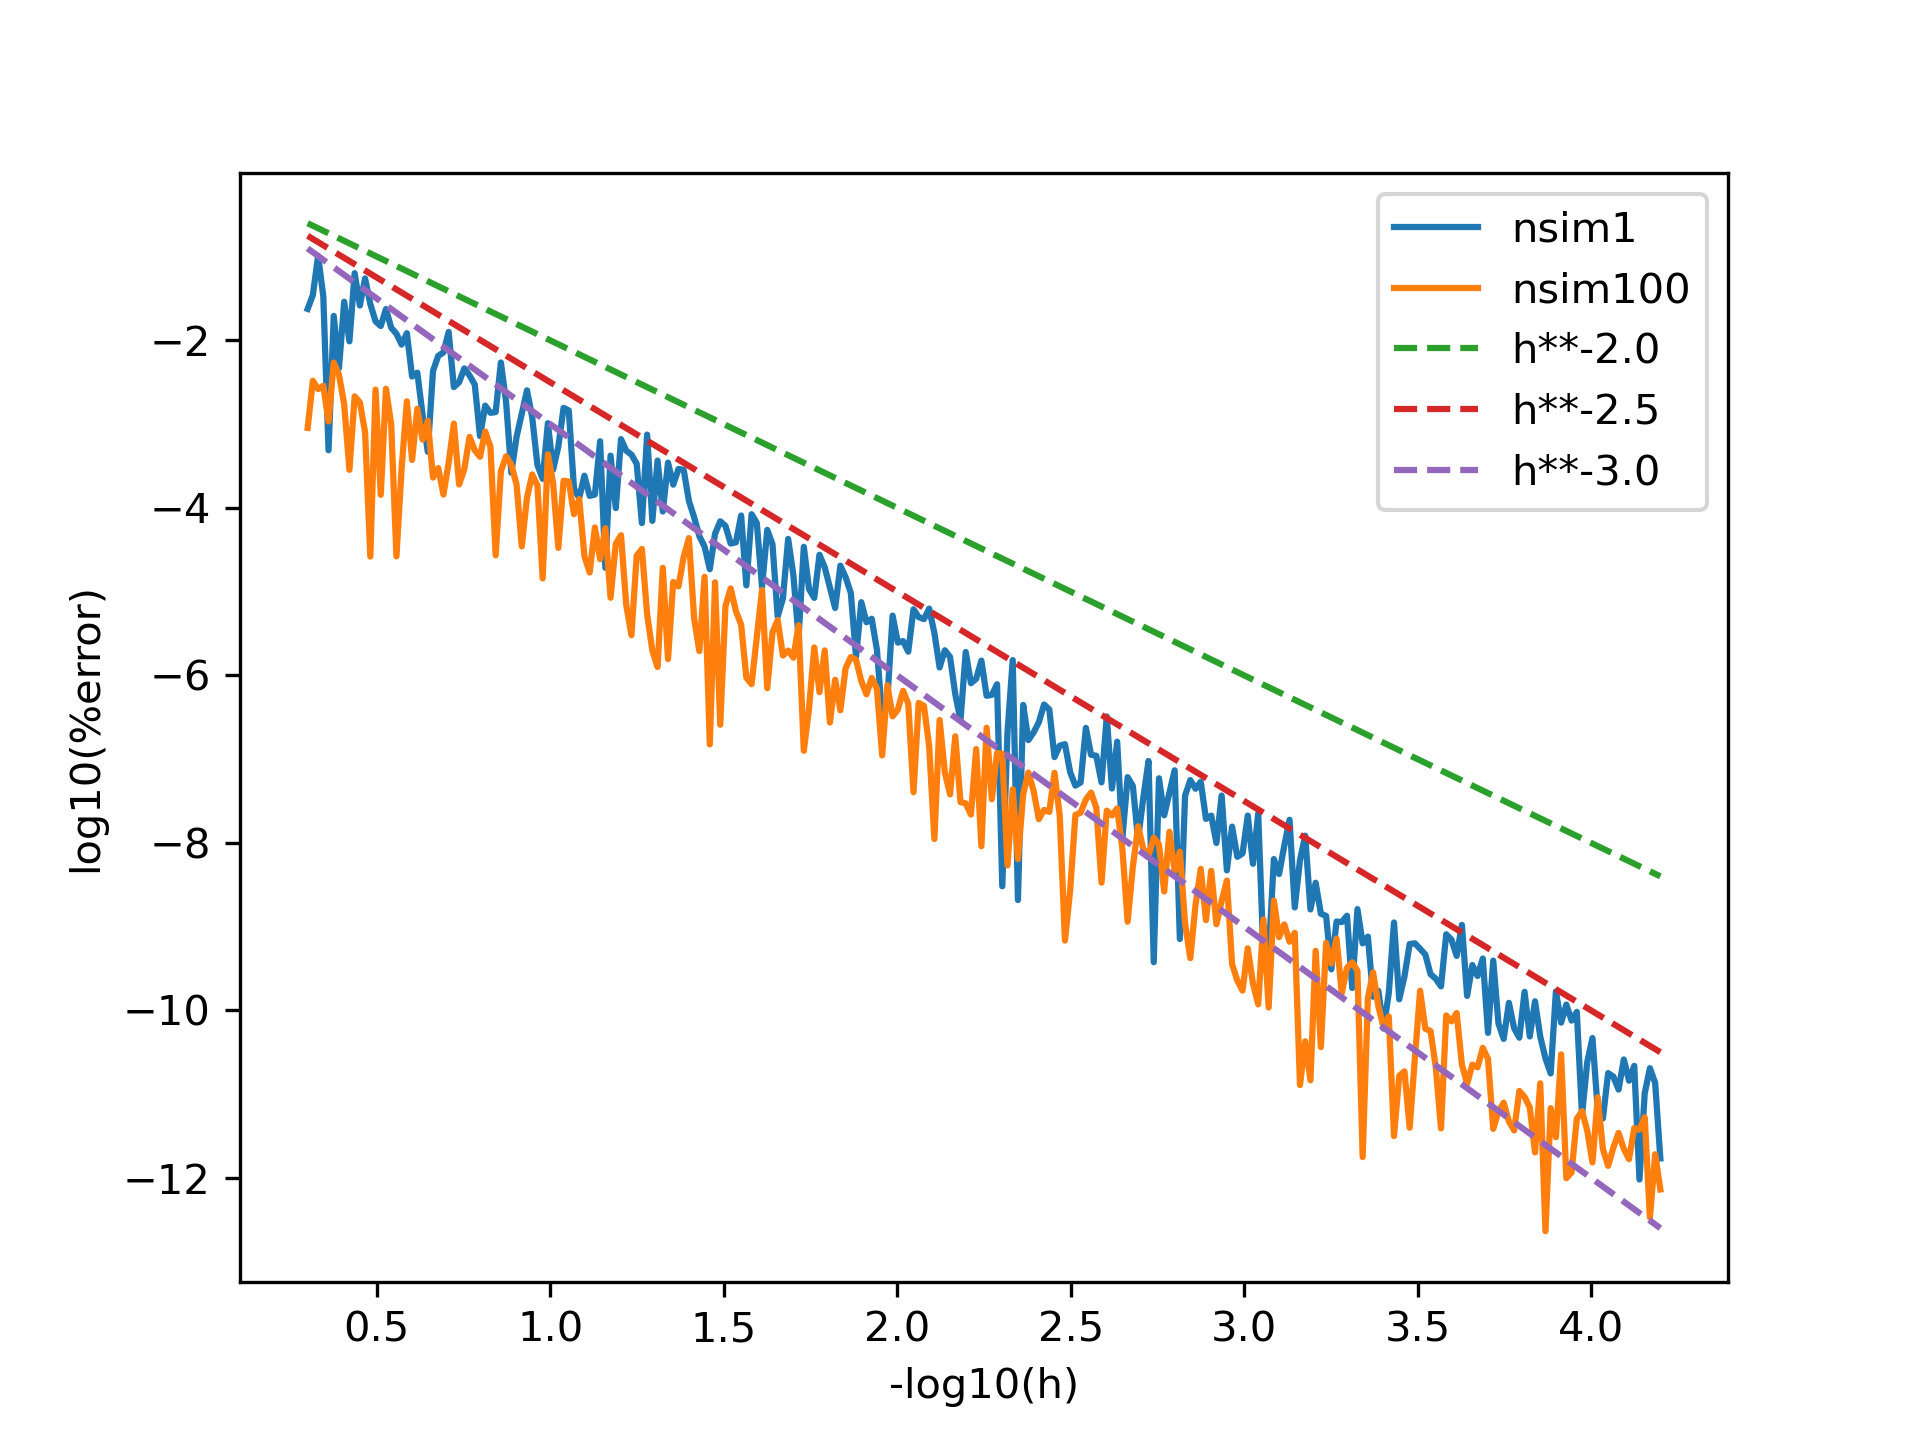
\includegraphics[width=0.8\textwidth]{plots/CV RRMC IVP.png}
        \caption{Log-log plot of the error for example
            \ref{ex:CV RRMC IVP} at $Y(10)$.}
        \label{fig:CV RRMC IVP}
    \end{figure}
\end{example}

\begin{related}[CV RRMC]
    \cite{daun_randomized_2011} similarly uses control variates to achieve
    a higher order of convergence.
\end{related}

Similar to explicit solvers, RRMC performs poorly on stiff problems.
We attempted to make RRMC more like implicit solvers but this proved difficult.
Instead, we think that an approach more like exponential integrators
is more viable. We experimented with Diagonal RRMC in this direction with
little success.

\begin{definition}[Diagonal RRMC] \label{def:DRRMC}
    Consider a general linear ODE IVP problem:
    \begin{equation}
        x' = Ax+g, \quad x(0)= x_{0}.
    \end{equation}
    Sometimes repeatedly multiplying by $A$ is unstable.
    Diagonal RRMC adds a positive diagonal matrix $D$
    to $A$ and hopes that it stabilizes.

    \begin{equation}
        x' + Dx = (A+D)x+g.
    \end{equation}

    The following integral equation can be derived by using integrating factor:

    \begin{equation}\label{eq:int eq DRRMC}
        x(t)= e^{D(t_{n}-t)}x(t_{n}) + \int_{t_{n}}^{t} e^{D(s-t)}(A(s)+D)x(s)ds+\int_{t_{n}}^{t} e^{D(s-t)}g(s)ds.
    \end{equation}

    Remember that the exponential of a diagonal matrix is the exponential of its elements.
    The recursive integral has the following trivial control variate:

    \begin{equation}\label{eq: CV DRRMC}
        \int_{t_{n}}^{t}  e^{D(s-t)}(A(t_{n})+D)x(t_{n})ds = D^{-1}(I-e^{D(t_{n}-t)})(A(t_{n})+D)x(t_{n}).
    \end{equation}

    Note that $D$ may be chosen differently for every outer recursion.
\end{definition}

\begin{example}[DRRMC] \label{ex:DRRMC}
    Consider:
    \begin{equation}
        x'= Ax, x(0)=
        \begin{bmatrix}
            1 \\
            0
        \end{bmatrix}.
    \end{equation}

    With

    \begin{equation}
        A = \begin{bmatrix}
            0     & 1     \\
            -1000 & -1001
        \end{bmatrix}.
    \end{equation}

    This has the following solution:

    \begin{equation}
        x(t) = \frac{1}{999}
        \begin{bmatrix}
            -  e^{-1000t}+ 1000 e^{-t} \\
            1000 e^{-1000t}- 1000e^{-t}
        \end{bmatrix}.
    \end{equation}

    We choose $D$ fixed over all outer recursions:

    \begin{equation}
        D = \begin{bmatrix}
            1 & 0    \\
            0 & 1000
        \end{bmatrix}.
    \end{equation}

    We make the convergence plot for this example with
    (\ref{eq:int eq DRRMC}) with control variate
    (\ref{eq: CV DRRMC}) implemented with recursion in recursion
    on Figure \ref{fig:DRRMC}.

    \begin{figure}[h!]
        \centering
        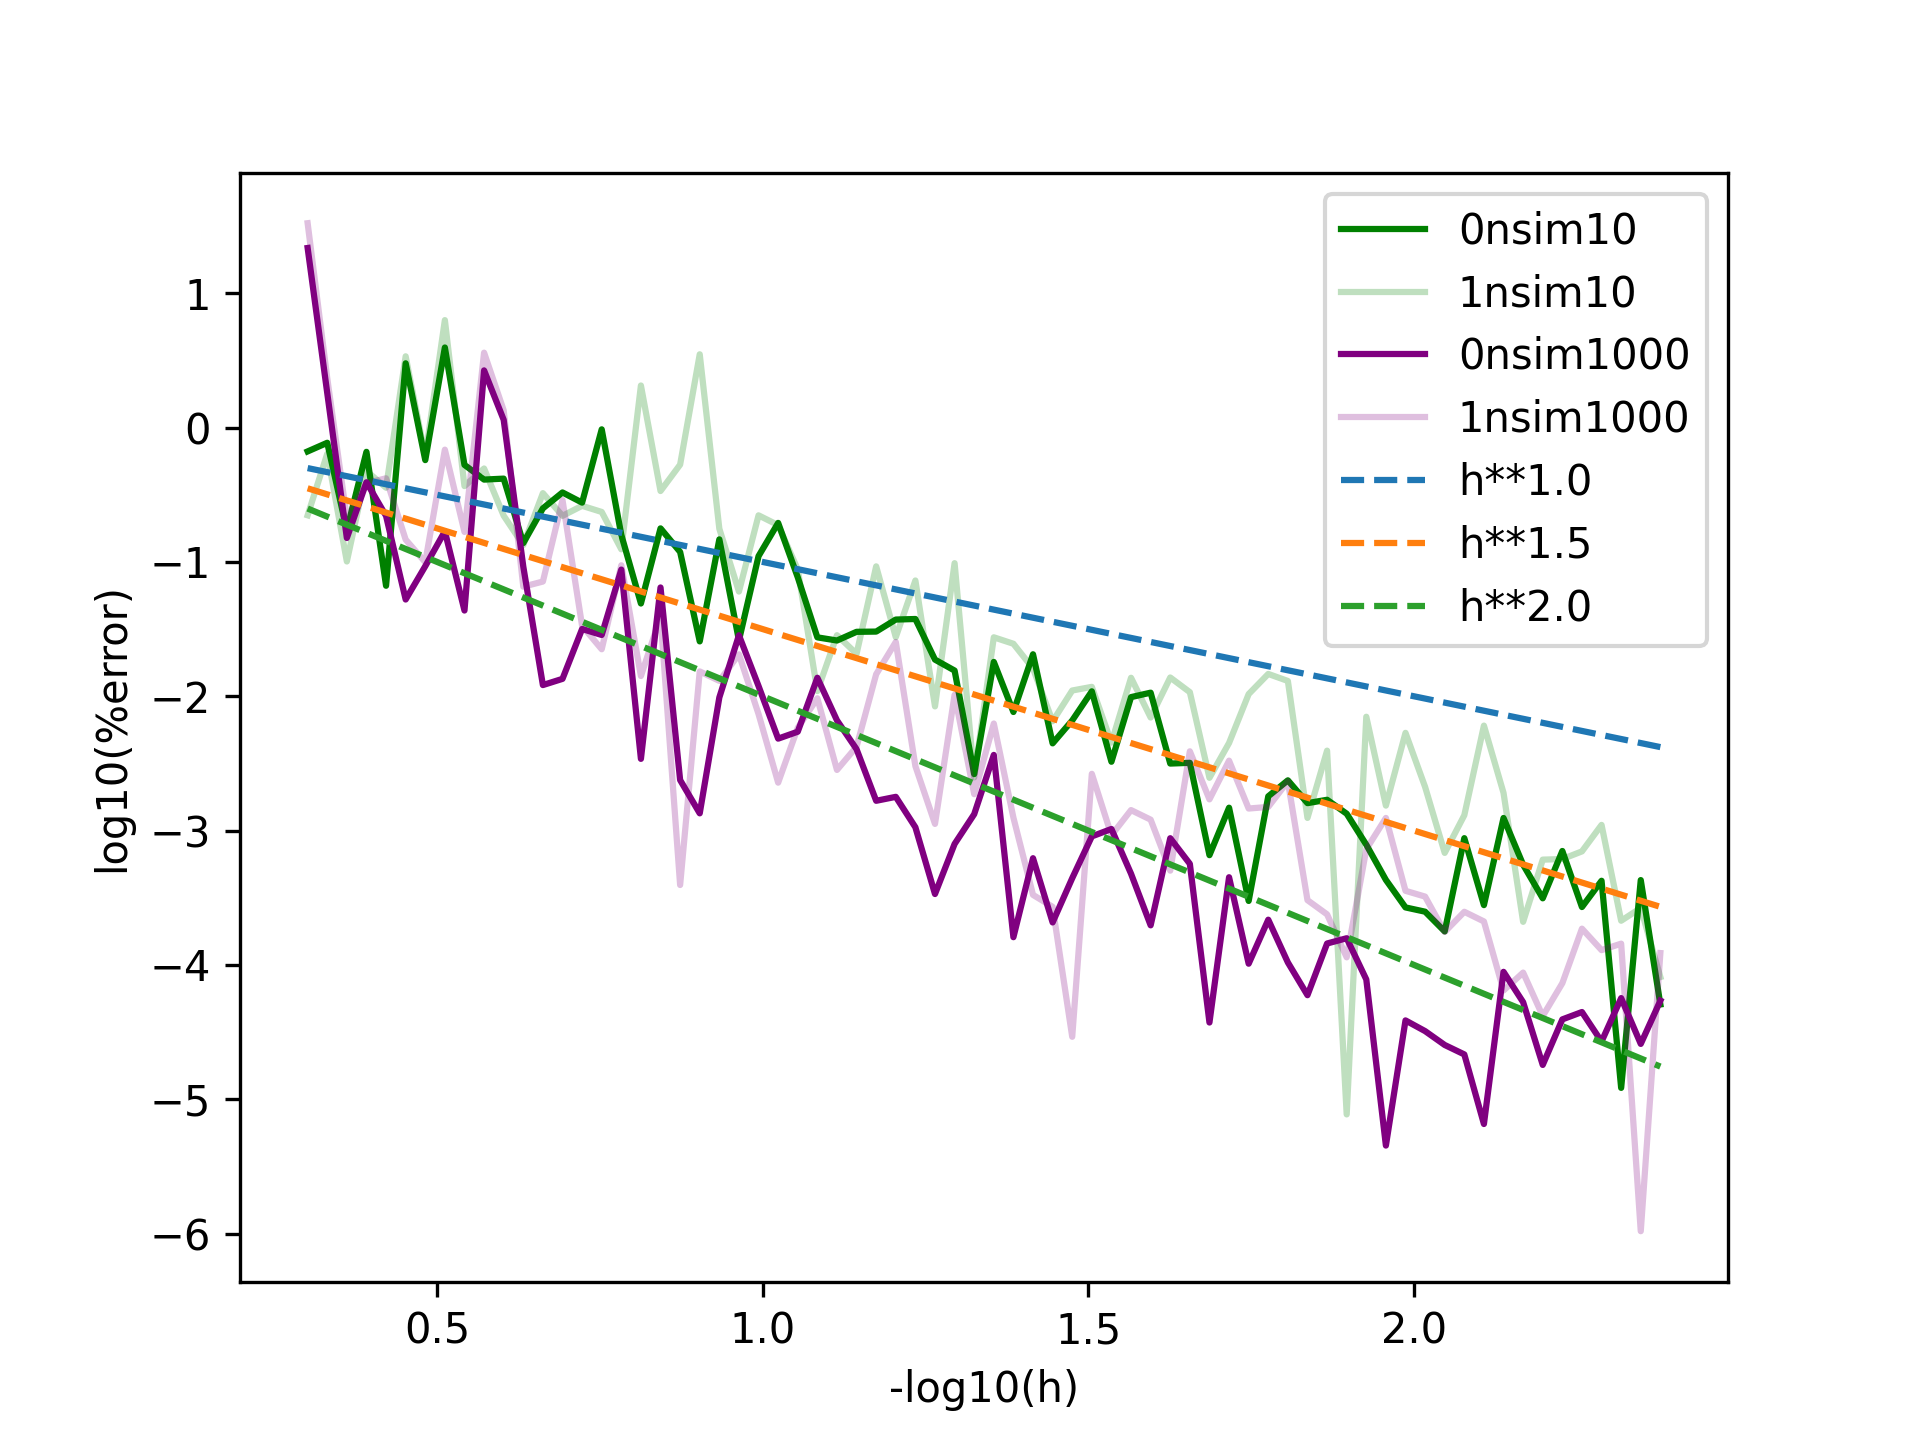
\includegraphics[width=0.8\textwidth]{plots/DRRMC.png}
        \caption{Log-log plot of the error of example \ref{ex:DRRMC}.
            We plotted the second component of the error transparent.
        }
        \label{fig:DRRMC}
    \end{figure}

\end{example}

\begin{related}[DRRMC]
    DRRMC is inspired by  $\bar{\sigma}$ parameter in \cite{sawhney_grid-free_2022} but
    instead of importance sampling, we use control variates to deal with
    nonlinearity introduced by the exponential because it needs to work over
    an entire vector at the same time.
\end{related}

\section{Limitations and Future Work}

Our goal for this thesis was to learn about and explore different Monte Carlo techniques.
We ended up limiting the scope to unbiased linear ODE solvers. In this direction,
there is still much obvious work to be done. \\

We think that understanding and optimizing unbiased and deterministic linear ODE solvers
is the key to developing better randomized ODE/PDE solvers.
Randomized ODE/PDE solvers are useful for cases with little structure
where the advantage of IBC is significant or in the case of a linear trade-off
between cost and variance is close to optimal. \\


Besides that, it is sometimes convenient to have low-bias access to solutions of
ODEs. For example, when integrating over a high dimensional parametric ODE problem
we would need unbiased solutions to do MC integration. The following example is
a toy problem where unbiased estimates are convenient.

\begin{example} \label{ex:random ode}
    Consider the following parametric IVP:
    \begin{equation}\label{eq:random ode}
        y_t = ay, \quad y(0)=1,
    \end{equation}
    with $a$ a parameter. The solution to this problem is given by
    $y(t,a) = e^{ta}$. Imagine we have a belief about $a$ quantized
    in the following way $a\sim U$. If we want
    to estimate $E[y(t, U)]$ or in a more general case
    $E[f(y(t, U))]$ with $f$ analytic directly
    we need samples of $y(t,U)$. If we don't have a solution for the parametric IVP
    we can't sample $y(t,U)$ instead, we use unbiased estimates ($Y(t,u)$) of samples ($y(t,u)$)
    of $y(t, U)$ in the following
    way using the total law of expectation:

    \begin{align}
        E[f(y(t,U))] & = E[f(y(t,u)) \mid U=u]     \\
                     & = E[f(E[Y(t,u)]) \mid U=u].
    \end{align}

    To estimate $E[f(E[Y(t,u)]) \mid U =u]$, we use the approach outlined in
    example \ref{ex:exp int}. For this example,
    we can compute the first two moments of $y(t, U)$:
    \begin{align}
        E[y(t,U)]      & = \frac{e^t}{t} - \frac{1}{t},      \\
        E[y^{2}(t, U)] & = \frac{e^{2t}}{2t} - \frac{1}{2t}.
    \end{align}
\end{example}

\begin{pythonn}[implementation of example \ref{ex:random ode}]
    \pythoncode{python code/random_ODE.py}
\end{pythonn}

\vspace{0.5cm}

While writing this thesis, we came up with a better way to sample the time process.
The time process we used is based on example \ref{ex: russian roulette}.
There are a few ways to generalize that example for example using a linear function
instead of an exponential. An issue is the lack of control over the stationary
distribution of the time process see Figure \ref{fig:russian roulette}.

\begin{figure}[h!]
    \centering
    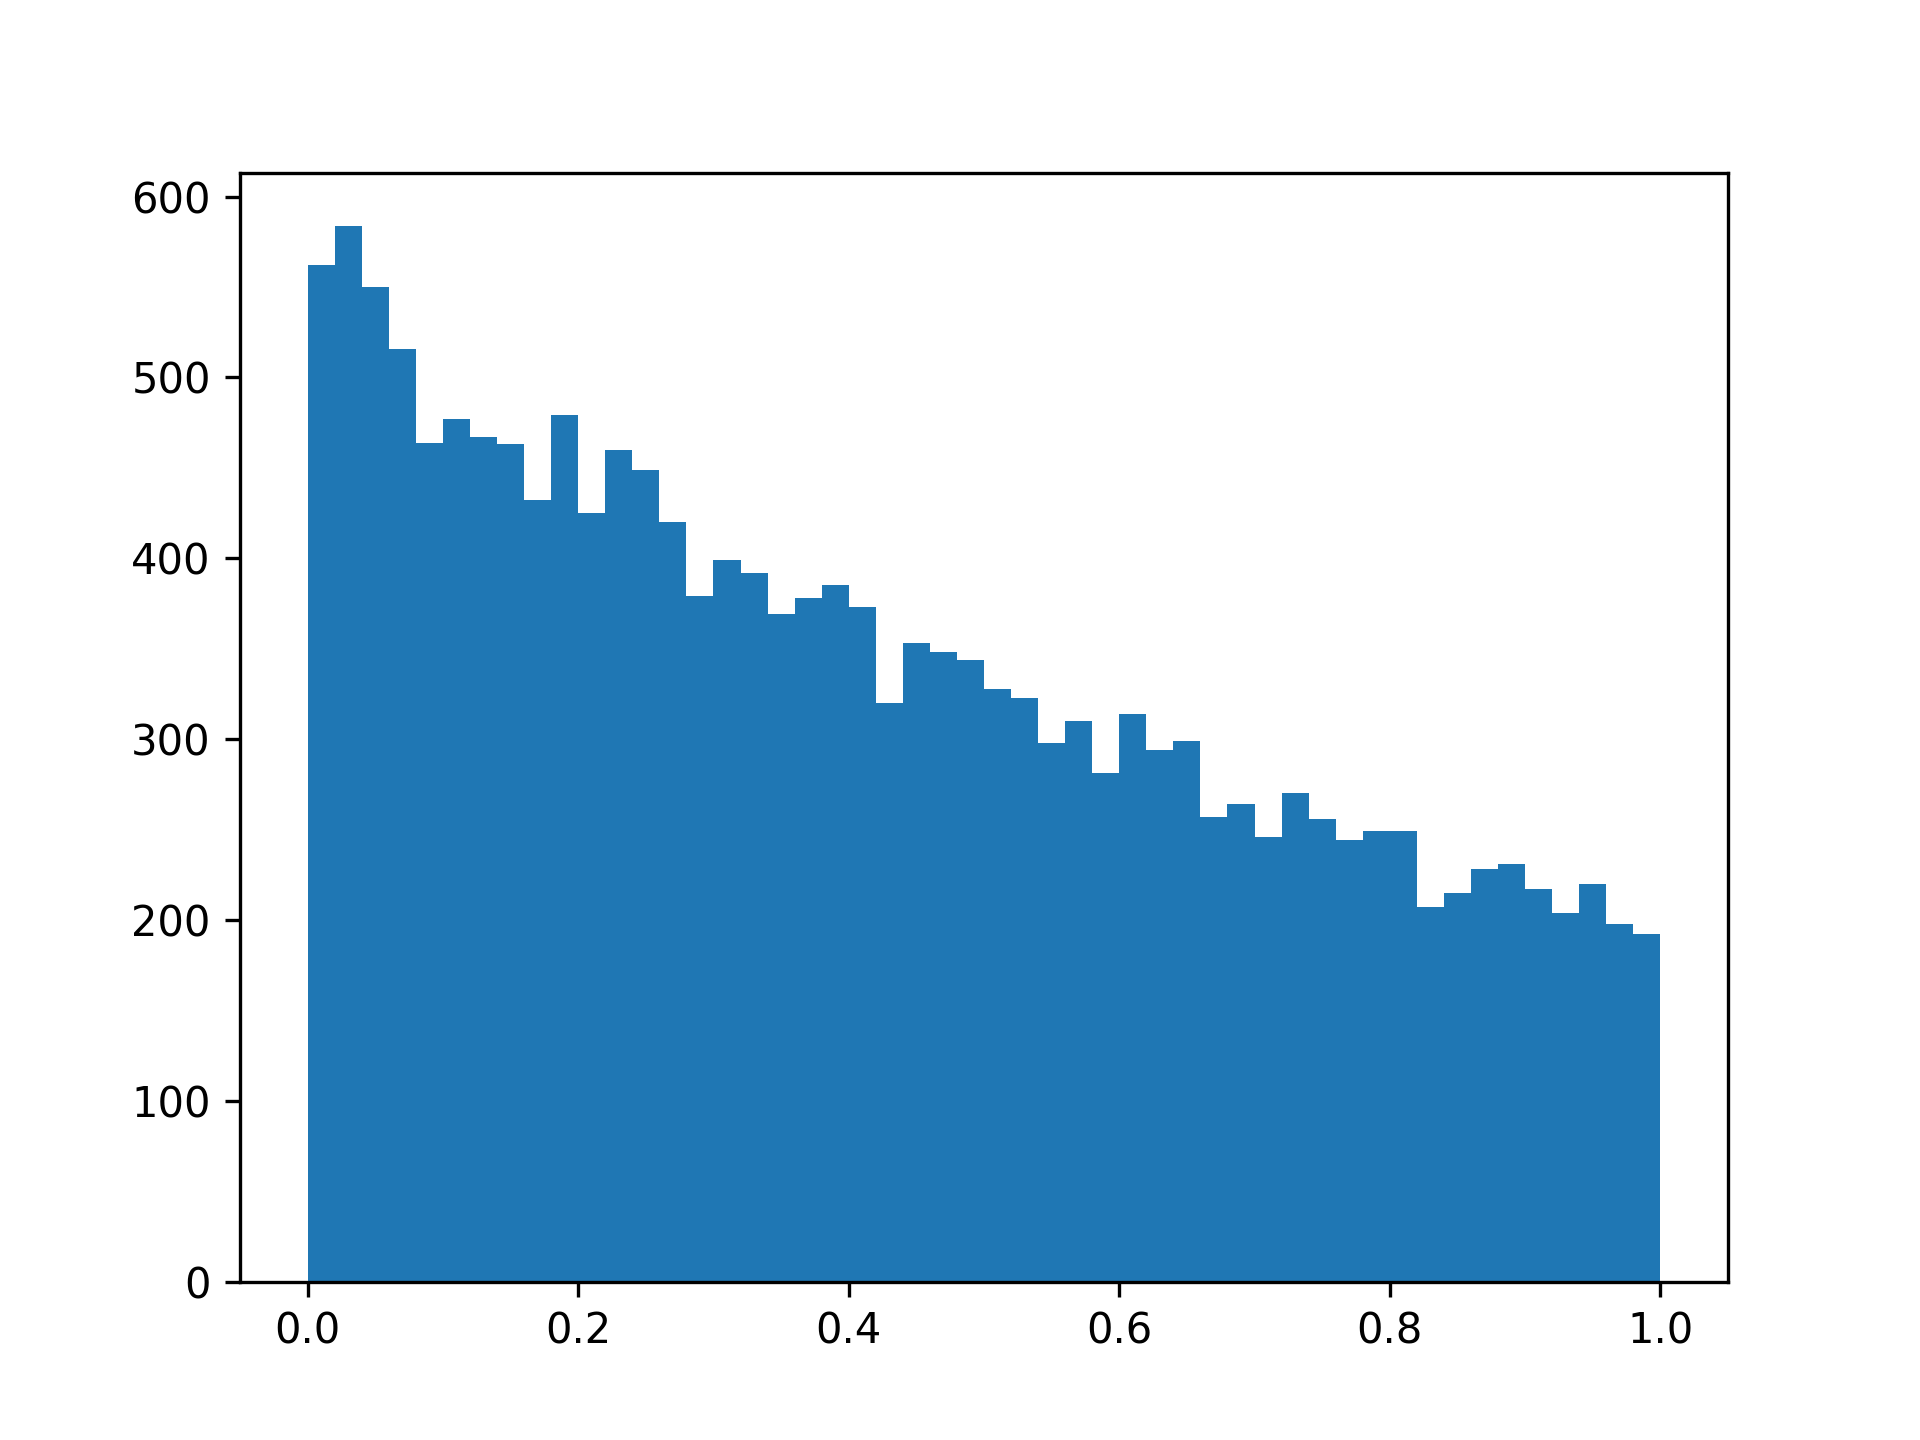
\includegraphics[width=0.8\textwidth]{plots/time proces.png}
    \caption{This histogram depicts how the points
        on Figure \ref{fig:russian roulette} are distributed over time
        excluding $t=1$.}
    \label{fig:time proces}
\end{figure}

What we have in mind is using a Poisson point process
that samples forwardly with the corresponding exponential distribution and
Russian roulettes when out of range. This way the stationary distribution
is controlled by the intensity of the Poisson process and the amount
of recursion calls (for constant intensity) are Poisson distributed.\\

Besides the time process, the following could be developed: the way control
variates are constructed, the type of control variates, adaptive schemes,
freezing less important terms in the recursion in recursion or Russian rouletting
them into reasonable approximations, error estimates based on variance in the
inner recursion, etc. \\

To deal with stiff problems in an unbiased way we would bet on exponential integrators
type of methods. The biggest obstacle to implementing them like diagonal RRMC is getting
unbiased estimates of $e^{A(t-s)} y(s)$ type of expressions. In the case
of a big matrix $A$ we think it would be important use unbiased sparsifaction
see \cite{sabelfeld_sparsified_2009}.
Initially, we came
up with example \ref{ex:exp int} but some time later we found
the paper from NVIDIA \cite{kettunen_unbiased_2021} that optimizes that example.
Closely related to this is directly estimating the Magnus expansion
where expressions like $e^{\int_{0}^{\Delta t} A(s)ds}  y(0)$ are needed. In this
case \cite{kettunen_unbiased_2021} doesn't address using the smoothness
of $A(s)$ which is needed for optimal IBC. \\

One of the elements that is lacking in our findings is rigor.  We think
that RMC for IVPs is an informal way to think of an unbiased estimate of
the Von Neumann series to the corresponding Volterra integral equation.
\cite{ermakov_monte_2019} has theorems (Theorem $1$ and $2$) that these
estimates have finite variance and even an expression for it.
Before being aware of \cite{ermakov_monte_2019} we
also derived a similar expression (probably with mistakes)
by using the law of total variance similar to (16) in \cite{rath_ears_2022}.\\
We think that proving optimal IBC for control variates + RRMC is doable
but tedious. \cite{daun_randomized_2011} has a proof for optimal IBC for their algorithm
in the biased non-linear case. The proof we have in mind is using a lower-bound on IBC
from integration and proving it gets achieved.\\

Optimal IBC isn't everything. Optimal IBC doesn't mean optimized. An algorithm that
uses $1000$ times more function calls has the same IBC. Besides that, the computational goal
may not fit well in the framework of IBC. We really like
\cite{becker_learning_2022} which uses deep learning to go outside
the IBC framework, the focus is more on multiple fast inferences where
a big precomputation is allowed.
IBC also doesn't take into account how
parallel computations are. Given infinite parallel resources it would make sense
to stop decreasing variance by reducing the step size and splitting the final estimator.
All the communication that is needed then is averaging the final estimator. We conjecture
that in such an estimator the wall time at risk would increase logarithmically with splitting
size.  \\

Another topic that could be investigated is only estimating $1$ component of the solution.
It is not obvious if this is always possible but due to the Feynman-Kac formula,
it seems possible for a space discretization of the heat equation.
We made the following informal partial derivation for the Feynman-Kac formula
in the case heat equation
to understand why and what makes point estimators possible.

Discretize the heat equation ($u_{t} = u_{xx}$)
with a regular rectangular mesh that includes $(x,t)$ with equally
spaced intervals over space and time ($\Delta x, \Delta t$) with
the corresponding difference equation:

\begin{equation}
    \frac{u(x,t)-u(x,t-\Delta t)}{\Delta t} = \frac{u(x + \Delta x,t)-2 u(x,t) +u(x - \Delta x,t)}{\Delta x^{2}} .
\end{equation}

Isolate $u(x,t)$:

\begin{equation} \label{eq:discrete iso heat equation}
    u(x,t) =
    \frac{\Delta t}{ 2 \Delta t + \Delta x^{2}}
    \left(
    u(x+\Delta x,t)+u(x-\Delta x,t)
    \right) +
    \frac{\Delta x^{2}}{ 2 \Delta t + \Delta x^{2}}
    \left(
    u(x,t-\Delta t)
    \right).
\end{equation}

Now comes the essential step in the derivation.
Because $u(x+\Delta x,t) \approx u(x-\Delta x,t) \approx u(x,t-\Delta t) \approx$
right-hand side of (\ref{eq:discrete iso heat equation}) we may Russian roulette
to remove branching recursion and generate a recursion path instead of a tree.
\begin{equation} \label{eq:RRVE discrete heat equation }
    Z(x,t) =
    \begin{cases}
        Z(x+\Delta x , t)  & \text{ with chance  } \frac{\Delta t}{ 2 \Delta t + \Delta x^{2}}     \\
        Z(x-\Delta x , t)  & \text{ with chance  } \frac{\Delta t}{ 2 \Delta t + \Delta x^{2}}     \\
        Z(x, t - \Delta t) & \text{ with chance  } \frac{\Delta x^{2}}{ 2 \Delta t + \Delta x^{2}}
    \end{cases}
\end{equation}

Taking the limit
makes the discrete solution converge to the real solution.
For (\ref{eq:RRVE discrete heat equation }) the limit
makes the recursion path go to Brownian motion. We won't treat
how to stop the recursion with boundary conditions.


\newpage
\begin{abstract}
    Deze scriptie onderzoekt unbiased Monte Carlo methoden voor
het oplossen van lineaire gewone differentiaalvergelijkingen met het
oog op partiële differentiaalvergelijkingen.
De voorgestelde algoritmes maken gebruik van de geschikte
combinatie van Monte Carlo technieken. Deze Monte Carlo technieken
worden geïntroduceerd met voorbeelden en code.
\end{abstract}

\printbibliography
\newpage

\end{document}

% Base your answers on the thesis.  
% You are expert in solving ODEs, WoS, IBC, PDEs giving feedback.
%
% Answer as a markdown file.
% Use subnumerings in mark down form in numbering the question 
% that works in a markdown file and use different headers. Like this: 
%
% # Content tests
% ##  0.1. How does the main algorithm work of the thesis?
% answer
%
% Here are the questions : 
% # Content tests
% 0.1. How does the main algorithm work of the thesis?
% 0.2. What is the biggest limitation of the main algorithm of the thesis?
% 0.3. How important is coupled splitting to the thesis?
% 0.4. How does Stein's paradox pop up in the thesis? (see subsection on MC integration)
% 0.5. Rate the language of the thesis.
% 0.6. List the 5 unclearest parts of the thesis.
% 0.7. What is special about the Monte Carlo trapezoidal rule?
% 0.8. What is the main advantage of the primary motivating work? 
% 0.9.  How does the thesis define Russian Roulette?
% 0.10. How does the thesis define control variates?
% 0.11. Summarize the approach for exponential of the expectance in the unbiased non-linearity section.
% 0.12. How does the thesis define tail recursion?
% 0.13. How does the thesis define Green's functions? 
% 0.14. Summarize convergence behavior of the main algorithm.
% 0.15. List your 5 favorite/intrestring parts of the thesis.
% 0.16. What seem to be missing in the thesis?
% 0.17. Any abbreviation that should/shouldn't be used?
% 0.18. List 5 inaccuracies things in the thesis.
% 0.19. List 5 controversial things in the thesis.
% 0.20. List 5 suggestions to improve the thesis.
%
% # Feedback 1
% 1.1 Does the thesis differentiate between the original contributions and prior work? 
% 1.2 Does the thesis has a good overview?
% 1.3 Does the thesis has a good conclusion?
% 1.4 Does everything gets defined in the thesis?
% 1.5 Are there symbols that don't get defined in the thesis?
% 1.6 What are the advantages of the solvers in the subsection of initial value problems 
% compared to classical solver?
% 1.7 Are the explanations for the graphs in the thesis sufficient?
% 1.8 Do equations, examples, definition, etc get referenced with consistent notation?
% 1.9 List 2 uncommon abbreviations that don't get introduced the first time they get used. 
%
% # Feedback 2
% 2.1 Has the elementary theory of Monte Carlo been covered in the thesis?
% 2.2 In the subsection of recursive Monte Carlo why is there indefinite 
% recursion?
% 2.3 Does the thesis give the necessary references to concepts?
% 2.4 Does additive branching gets explained clearly?
% 2.5 What is the Russian roulette rate ?
% 2.6 Does the local truncation error get defined ?

% # Requirements
% 3.1 Title Page: Does the thesis have a title page? 
% 3.2 Table of Contents: Does the thesis include a table of contents?
% 3.3 Introduction: 
%     Does the introduction provide a clear context for the research?
%     Is the problem statement or research question clearly formulated in the introduction?

% 3.4 Exposition:
%     Is the argumentation detailed and logical, leading to the final result of the research?
%     Is the substructure effectively used to organize and clarify the content within the exposition?

% 3.5 Dutch Summary:

%     Does the thesis include a Dutch summary?
%     Is the Dutch summary concise, effectively summarizing the main points of the thesis within the specified page limit?

% 3.6 Bibliography:

%     Is the bibliography section present and well-structured?
%     Are all the cited sources accurately listed in the bibliography according to the specified citation style?

% 3.7 Layout and Readability:
%   - Is the layout designed to enhance readability, including appropriate font, line spacing, and paragraph structure?
%   -  Is the use of headings, subheadings, and other formatting elements consistent and effective in guiding the reader through the content?

% 3.8 Language Quality:
% - Is the language used throughout the thesis refined and well-crafted?
% - Are grammar, spelling, and punctuation accurate?

% 3.9 Results and Analysis:

% - Are the results presented clearly and comprehensively?
% - Is the analysis of the results thorough, and do the conclusions logically follow from the data?

% 3.10 Argumentation and Coherence:

% - Is there a clear and logical progression of ideas throughout the thesis?
% - Do transitions between sections and paragraphs enhance the overall coherence of the document?

% 3.11 Original Contribution:
% - Does the thesis make a unique and valuable contribution to the field of study?
% - Is there a clear statement about how the research fills a gap in existing knowledge?

% 3.12 Discussion and Implications:
% - Does the discussion section provide insights into the broader implications of the research findings?
% - Are any practical applications or future research directions suggested?

% 3.13 Clarity and Conciseness:
% - Is the writing style clear and concise, avoiding unnecessary jargon?
% - Are complex concepts explained in a way that is understandable to the intended audience?

% 3.14 Overall Contribution:
% - Does the thesis contribute significantly to the field's body of knowledge and understanding?
% - Is the thesis likely to be cited and referenced by others in the field?

